% Сборка: ./build.sh из этой директории либо ./part2/build.sh из корня.
\documentclass[11pt,a4paper]{article}
\usepackage[round,authoryear,comma]{natbib}
\usepackage[russian]{optimstyle}
\usepackage{tabularx,pifont,calc,xurl,fontawesome5,nicefrac}
\usepackage{placeins}
\usepackage{tikz}
\usetikzlibrary{arrows.meta,positioning,shapes.geometric,calc}
\colorlet{cheapline}{optimBlue}
\colorlet{cheapfill}{optimBlue!5!white}
\newcommand{\R}{\mathbb R}
\newcommand{\E}{\mathbb E}
\newcommand{\ip}[2]{\langle #1,#2\rangle}
\newcommand{\norm}[1]{\lVert#1\rVert}
\newcommand{\eps}{\varepsilon}
\newcommand{\Fs}{f^\ast}
\DeclareMathOperator{\argmin}{arg\,min}
\DeclareMathOperator{\dist}{dist}
\newcommand{\by}[2]{\mathrel{\underset{#2}{#1}}}
\newcommand{\bypad}[3]{\mathrel{\underset{\mathmakebox[\widthof{$\scriptstyle#3$}]{#2}}{#1}}}
\newcolumntype{P}[1]{>{\raggedright\arraybackslash}p{#1}}
\newcolumntype{Y}{>{\raggedright\arraybackslash}X}
% Expand generated rows directly inside tabular, before booktabs rules.
\makeatletter
\newcommand{\experimentrows}[1]{\@@input #1 }
\makeatother
\setlist[itemize]{label=$\vartriangleright$}
\algrenewcommand\algorithmicloop{\textbf{повторять}}
\algrenewcommand\algorithmicwhile{\textbf{пока}}
\relpenalty=10000 \binoppenalty=10000 \emergencystretch=10em
\BeforeBeginEnvironment{theorem}{\Needspace{6\baselineskip}}
\BeforeBeginEnvironment{lemma}{\Needspace{6\baselineskip}}
\BeforeBeginEnvironment{proposition}{\Needspace{6\baselineskip}}
\BeforeBeginEnvironment{definition}{\Needspace{6\baselineskip}}
\BeforeBeginEnvironment{assumption}{\Needspace{7\baselineskip}}
\tcbset{optimassumption/.style={optimbox,colback=optimGreen!5!white,
  colframe=optimGreen!45!white,borderline west={1.2pt}{0pt}{optimGreen}}}
% Keep subsection headings with the following proof or displayed formula.
\pretocmd{\subsection}{\Needspace{8\baselineskip}}{}{}
\renewcommand{\optimtitlefont}{\fontsize{16}{21}\selectfont\bfseries\boldmath}
\title{«Спуск с Эвереста», часть~II\texorpdfstring{\\[3pt]}{: }
Оракульная сложность минимизации суммы\texorpdfstring{\\}{ }
выпуклых \texorpdfstring{$(L_0,L_1)$}{(L0,L1)}-гладких функций\texorpdfstring{\thanks{Английская версия статьи: \url{https://arxiv.org/abs/2611.04171}.}}{}}
% Как в первой части: в шапке только имена; аффилиации и почты вынесены в сноски.
\author{%
  Михаил Рудоманов\thanks{MIRIAI, Moscow Independent Research Institute of Artificial Intelligence, Москва, Россия. \email{rudomanov.ma@phystech.edu}.}\,\thanks{Равный вклад.}\quad
  Иван Фомин\thanks{Яндекс, Москва, Россия. \email{ash-ivanfomin@yandex-team.ru}.}\,\footnotemark[3]\\[4pt]
  Александр Владимирович Гасников\thanks{Университет Иннополис, Иннополис, Россия. \email{gasnikov@yandex.ru}.}\quad
  Федор Сергеевич Стонякин\thanks{КФУ им.~В.\,И.~Вернадского, Симферополь, Россия. \email{fedyor@mail.ru}.}}
\hypersetup{pdfauthor={Михаил Рудоманов, Иван Фомин, Александр Владимирович Гасников, Федор Сергеевич Стонякин}}
\date{}
\keywords{$(L_0,L_1)$-гладкость, обобщённая гладкость, минимизация суммы функций,
оракульная сложность, нижние оценки, ускоренные методы, уменьшение дисперсии.}
\begin{document}
\begingroup
\makeatletter
\renewcommand{\@fnsymbol}[1]{\ensuremath{\ifcase#1\or *\or\spadesuit\or\text{\tiny\faMountain}\or\clubsuit\or\dagger\or\ddagger\fi}}
\let\origmakefntext\@makefntext
\long\def\@makefntext#1{\rightskip\z@\@plus3em\relax\origmakefntext{#1}}
\makeatother
\maketitle
\endgroup
\begin{abstract}
Рассматривается минимизация среднего $n$ выпуклых $(L_0,L_1)$-гладких
функций: норма гессиана каждой из них ограничена аффинной функцией
нормы её градиента. Предполагаются известными верхняя граница $R$ расстояния
от начальной точки до точки минимума и верхняя граница $\delta$ разности между минимумом среднего и средним значением
инфимумов слагаемых. Получены верхняя и нижняя оценки оракульной сложности
достижения точности $\varepsilon$ по функции в среднем. С точностью до логарифмических множителей обе оценки имеют порядок
\[
 n\bigl(1+(L_1R)^{2/3}\bigr)
 +\sqrt{\frac{n(L_0+L_1^2\delta)R^2}{\varepsilon}+n(L_1R)^2}.
\]
Верхняя оценка достигается предложенным методом YETI. Метод использует
идеи ускоренных проксимальных методов и методов уменьшения дисперсии,
а также эвристику для выбора дополнительных точек.
Число обращений эвристики к оракулу ограничено, что позволяет
сохранить верхнюю оценку общего числа запросов до достижения нужной точности.
В экспериментах YETI сравнивается с методами первого порядка
на синтетических задачах и задачах пуассоновской регрессии.
Отдельно проверяются критерий остановки и влияние эвристики.
Нижняя оценка получена явным построением
семейств задач, трудных для любого метода первого порядка.
\end{abstract}

% Использование языковых моделей
\begin{tcolorbox}[
  optimbox,
  colback=optimBlue!3!white,
  colframe=optimBlue!40!white,
  borderline west={1.4pt}{0pt}{optimBlue},
  top=7pt,bottom=7pt
]
\small
\noindent\textbf{Использование языковых моделей.}\enspace
При получении теоретических результатов настоящей работы использовались
модели \textit{Codex Astra 6} и \textit{Claude Opus 5.5}.
Они также применялись при подготовке и вёрстке рукописи и для перевода
исходного текста на английский язык.
Однако каждая строка статьи, включая каждое утверждение, каждое
доказательство и каждое вычисление, лично отредактирована и проверена
авторами. Ответственность за корректность всех математических утверждений,
доказательств и выводов несут исключительно авторы работы.
\end{tcolorbox}

\section{Введение}\label{sec:intro}

Мы рассматриваем задачу минимизации суммы функций
\[
 f(x)=\frac1n\sum_{i=1}^n f_i(x)\to\min_{x\in\R^d}.
\]
Задачи такого вида возникают при минимизации эмпирического риска
в машинном обучении, где $f_i$ --- функция потерь на $i$-м объекте
обучающей выборки \citep{shalev2014understanding,bottou2018optimization}.
В федеративном и распределённом обучении слагаемое $f_i$ --- это функция
потерь на данных $i$-го устройства или вычислительного узла
\citep{mcmahan2017communication}. Градиент одного слагаемого часто вычисляется
существенно дешевле полного градиента. Поэтому сложность методов мы измеряем
числом обращений к оракулу, который возвращает значение и градиент одного слагаемого.

Для суммы $L$-гладких функций число обращений к оракулу позволяют сократить
методы уменьшения дисперсии \citep{johnson2013svrg,xiao2014proxsvrg}.
Они периодически вычисляют полный градиент $f$, а на остальных
шагах используют градиенты отдельных слагаемых $f_i$.
Нижние оценки для произвольных рандомизированных методов показывают,
какие зависимости от числа слагаемых и точности улучшить нельзя
\citep{woodworth2016finite}.

Однако условие $L$-гладкости не выполняется, например, для экспоненциальных
функций потерь. Условие $(L_0,L_1)$-гладкости введено в работе
\citet{zhang2019gradient}, чтобы объяснить успех методов
с клиппированием градиента. При обучении языковой модели на основе LSTM авторы
заметили, что локальная константа гладкости растёт вместе с нормой градиента.
Аналогичная зависимость обнаружена и при обучении трансформеров
\citep{crawshaw2022robustness}.
Условие $(L_0,L_1)$-гладкости как раз допускает такой рост кривизны.
Его обобщения и методы первого порядка для таких функций изучались
в работах
\citet{li2023generalized,gorbunov2024methods,vankov2025optimizing,tyurin2025unified}.
Для конечных сумм нужно учитывать одновременно и число слагаемых, и рост кривизны.
Например, в пуассоновской регрессии с логарифмической функцией связи
\citep{stanPoisson}
$f_i(x)=\exp(a_i^{\mathsf T}x)-b_i a_i^{\mathsf T}x$, где $b_i\ge0$,
гессиан не ограничен на всём пространстве, но
\[
 \norm{\nabla^2 f_i(x)}
 \le b_i\norm{a_i}^2+\norm{a_i}\norm{\nabla f_i(x)}.
\]
В задаче восстановления фазы по измерениям интенсивности используются потери
$f_i(x)=(\ip{a_i}x^2-b_i)^2$
\citep{candes2015wirtinger}. Здесь также приходится минимизировать конечную сумму
слагаемых с неограниченной кривизной.
Ещё один пример --- экспоненциальные потери в задаче классификации
\citep[пример~1.5]{gorbunov2024methods}.
Во всех этих задачах при большом числе наблюдений вычислять полный градиент
может быть дорого, а сам градиент не является глобально липшицевым.
Поэтому нужны методы, которые учитывают рост кривизны и не вычисляют
градиенты всех слагаемых на каждом шаге. Ниже предполагается,
что функция $f$ достигает минимума, а расстояние до точки минимума, начальная невязка
и неоднородность слагаемых ограничены.

\paragraph{Особенность суммы функций.}
В рассматриваемой задаче каждое слагаемое удовлетворяет неравенству
\[
 0\preceq\nabla^2f_i(x)
 \preceq\bigl(L_{0,i}+L_1\norm{\nabla f_i(x)}\bigr)I.
\]
Даже в точке минимума среднего градиенты отдельных слагаемых могут быть
большими: равенство $\nabla f(x^\ast)=0$ означает лишь, что их сумма
равна нулю. Поэтому малость нормы полного градиента не влечёт малости
констант гладкости слагаемых, от которых зависят оценки методов уменьшения
дисперсии. Какова оракульная сложность минимизации суммы в этой ситуации?
Мы отвечаем на этот вопрос в настоящей работе.

\paragraph{Обозначения.} Через $\varepsilon>0$ обозначается требуемая точность решения задачи по функции: метод должен выдать точку $\hat x$, для которой $f(\hat x)-f^\ast\le\varepsilon$. Знак $\norm{\cdot}$ всюду означает евклидову норму вектора и спектральную норму матрицы, $[x,y]$ --- отрезок с концами $x,y\in\R^d$, $B(x,r)$ --- замкнутый шар радиуса $r$ с центром $x$. Сумму первых $k$ членов последовательности мы обозначаем соответствующей заглавной буквой: например, $A_k=a_1+\dots+a_k$ и $A_0=0$.


Для рандомизированных методов указанная точность требуется
в математическом ожидании. Все проекции евклидовы; через $\Pi_C$
обозначается проекция на непустое замкнутое выпуклое множество $C$.

\paragraph{Основной результат.}
Пусть слагаемые выпуклы, дважды непрерывно дифференцируемы и ограничены
снизу, а $n^{-1}\sum_iL_{0,i}\le L_0$. Начальную точку $x_0$ будем считать
нулевой: этого можно добиться сдвигом, относительно которого класс
задач инвариантен. Предполагается, что $f$ достигает минимума в точке
$x^\ast$, причём $\norm{x^\ast}\le R$ и $f(0)-f^\ast\le\Delta$.
При условиях теоремы~\ref{thm:main} верхняя и нижняя оценки сложности
имеют, с точностью до логарифмических множителей, порядок
\[
 n\bigl(1+(L_1R)^{2/3}\bigr)
 +\sqrt{\frac{n(L_0+L_1^2\delta)R^2}{\varepsilon}+n(L_1R)^2}.
\]
Здесь под сложностью понимается математическое ожидание числа запросов
значений и градиентов отдельных слагаемых в худшем случае,
достаточного для выполнения $\E[f(\hat x)-f^\ast]\le\varepsilon$.
Нижняя оценка справедлива для произвольных рандомизированных методов;
размерность задачи при этом не ограничена.
Точное определение класса и логарифмические множители приведены
в разделе~\ref{sec:setting}.

\paragraph{Замечание о логарифмических множителях.}
В верхней оценке скрыт множитель $\log^2N$, где $N$
из~\eqref{eq:complexity-parameters} растёт линейно по $\Delta/\varepsilon$.
В худшем случае, когда $\Delta$ экспоненциально велико по $L_1R$,
этот логарифм может иметь порядок $L_1R$, так что множитель $\log^2N$ может иметь порядок $(L_1R)^2$,
то есть давать дополнительный полиномиальный множитель.

Слагаемое $\sqrt{nL_0R^2/\varepsilon}$ известно из теории минимизации
суммы $L$-гладких функций \citep{woodworth2016finite}.
Слагаемое $n(L_1R)^{2/3}$ отражает число обращений к оракулу,
необходимое, чтобы приблизиться к минимуму из области, где градиенты
экспоненциально велики. Слагаемое
\[
 \sqrt{\frac{nL_1^2R^2\delta}{\varepsilon}+n(L_1R)^2}
\]
возникает из-за того, что кривизна слагаемых вблизи минимума
определяется их градиентами, которые могут оставаться большими даже в точке
минимума среднего.

\paragraph{Метод и эксперименты.}
Верхнюю оценку достигает метод YETI. При малой локальной кривизне
он выполняет ускоренный шаг, решая вспомогательную задачу методом SVRG,
а при большой --- проецирует вспомогательную точку на полупространство,
содержащее точку минимума. Кроме того, YETI использует эвристику
с ограниченным числом запросов к оракулу: она позволяет воспользоваться
удачными предложенными точками, не ухудшая теоретическую оценку.
В экспериментах YETI сравнивается с другими методами и проверяется
его критерий остановки.

\paragraph{Связь с известными методами.}
YETI использует ускоренную проксимальную схему
Монтейро--Свайтера \citep{ms2013} и идею адаптивного выбора
регуляризации без решения неявного уравнения на каждом шаге
\citep{carmon2022adaptive}. Локальная задача решается
проекционным вариантом SVRG. Ускорение за счёт приближённого решения
регуляризованных задач изучалось также в схеме Catalyst
\citep{lin2015catalyst,lin2018catalyst} и в работе
\citet{frostig2015}. В YETI выбор шага зависит от вычисляемой оценки
кривизны суммы: если эта оценка слишком велика, метод вместо шага строит
отделяющее полупространство. Оценка сложности учитывает запросы
и локального решателя, и эвристики.

Нижняя оценка опирается на принцип Яо \citep{yao1977}: трудная задача
выбирается случайно из конечного семейства, после чего проводится усреднение
по случайным величинам алгоритма. Скрытые координаты и распределение
информации по разным слагаемым продолжают известный подход к построению
нижних оценок для задач минимизации суммы \citep{woodworth2016finite}.
Для рассматриваемого класса мы применяем экспоненциальные
преобразования выпуклых цепочек и выбираем их параметры так,
чтобы выполнялись ограничения на $L_1$, $\delta$ и начальную невязку.

Настоящая статья продолжает нашу предыдущую работу \citet{rudomanov2026everest}, в которой
оракульная сложность этого класса найдена для одной функции ($n=1$):
её порядок равен $\sqrt{L_0R^2/\varepsilon}+L_1R$, а при малой
начальной невязке --- $\sqrt{L_0R^2/\varepsilon}+(L_1R)^{2/3}$.
Здесь рассматривается сумма функций, а оракул возвращает значение
и градиент лишь одного слагаемого, поэтому для получения верхней оценки
мы используем уменьшение дисперсии.
Результаты для одной функции
\citep{vankov2025optimizing,tyurin2026accelerated} относятся
к оракулу, вычисляющему полный градиент. В частности, оптимальность
метода \citet{tyurin2026accelerated} при достаточно малых $\varepsilon$ основана
на классической нижней оценке для гладкого подкласса и касается только
ведущего члена $\sqrt{L_0R^2/\varepsilon}$. Оптимальность слагаемого
$n(L_1R)^{2/3}$ для оракула, возвращающего градиент одного слагаемого,
из неё не вытекает.
Аналогично,
оценки для стохастических методов в случае общей точки минимума всех слагаемых
\citep{gorbunov2024methods}
не охватывают произвольную положительную неоднородность $\delta$.

\paragraph{Организация работы.}
Постановка задачи и основной результат приведены в разделе~\ref{sec:setting},
метод YETI и его анализ --- в разделах~\ref{sec:cheap}--\ref{sec:cheap-analysis},
основные эксперименты --- в разделе~\ref{sec:experiments}
(дополнительные эксперименты и их детали --- в приложении~\ref{app:experiments}), нижняя оценка ---
в разделе~\ref{sec:lower}. В основном тексте приведены
результаты и схема доказательства нижней оценки, а вспомогательные
доказательства и варианты метода вынесены в приложения. Сводная таблица
известных оценок приведена в приложении~\ref{app:literature}.

\section{Постановка задачи и основные оценки}\label{sec:setting}

Рассматривается функция $f=n^{-1}\sum_{i=1}^n f_i$ на $\R^d$.
Заданы $n\ge2$, $L_0,\delta\ge0$ и $L_1,R,\Delta,\varepsilon>0$.
Начальную точку считаем нулевой; этого можно добиться сдвигом координат.
Все общие предположения собраны ниже.

\begin{assumption}[компоненты]\label{asm:components}
Функции $f_i:\R^d\to\R$, $1\le i\le n$, выпуклы,
дважды непрерывно дифференцируемы и ограничены снизу.
\end{assumption}

\begin{assumption}[обобщённая гладкость]\label{asm:smoothness}
Известны числа $L_{0,i}\ge0$, для которых
\begin{equation}\label{eq:component-class}
 \begin{gathered}
 \norm{\nabla^2 f_i(x)}\le L_{0,i}+L_1\norm{\nabla f_i(x)}
 \quad(x\in\R^d,\ 1\le i\le n),\\
 \frac1n\sum_{i=1}^n L_{0,i}\le L_0.
 \end{gathered}
\end{equation}
\end{assumption}

\begin{assumption}[точка минимума]\label{asm:minimizer}
Существует точка минимума $x^\ast\in\argmin f$, для которой $\norm{x^\ast}\le R$.
Обозначим $f^\ast=f(x^\ast)$.
\end{assumption}

\begin{assumption}[начальная невязка]\label{asm:initial-gap}
Выполнено $f(0)-f^\ast\le\Delta$, причём $\Delta\ge2\varepsilon$.
\end{assumption}

\begin{assumption}[неоднородность]\label{asm:heterogeneity}
\begin{equation}\label{eq:problem-bounds}
 f^\ast-\frac1n\sum_{i=1}^n\inf_{x\in\R^d}f_i(x)\le\delta.
\end{equation}
\end{assumption}

\begin{assumption}[диапазон точностей]\label{asm:accuracy}
\begin{equation}\label{eq:nondegenerate}
 \frac{L_1^2R^2\delta}{\varepsilon}\ge3.
\end{equation}
\end{assumption}

\begin{definition}[класс задач]\label{def:class}
Через $\mathcal P_d$ обозначим множество наборов функций
$f_1,\ldots,f_n:\R^d\to\R$ и известных чисел $L_{0,1},\ldots,L_{0,n}$,
удовлетворяющих предположениям~\ref{asm:components}--\ref{asm:heterogeneity}.
\end{definition}

Предположение~\ref{asm:smoothness} ограничивает только среднее
чисел $L_{0,i}$; отдельные $L_{0,i}$ могут превышать $L_0$.
Нижнюю оценку достаточно построить на подклассе $L_{0,i}=L_0$.
Для $C^2$-функций ограничение на гессиан из предположения~\ref{asm:smoothness} эквивалентно
симметричной $(L_{0,i},L_1)$-гладкости
\citep[предположение~1.3, формула~(5)]{gorbunov2024methods}:
\[
 \norm{\nabla f_i(x)-\nabla f_i(y)}
 \le\Bigl(L_{0,i}+L_1\sup_{z\in[x,y]}\norm{\nabla f_i(z)}\Bigr)\norm{x-y}.
\]
Предположение~\ref{asm:heterogeneity} не требует знать ни $f^\ast$,
ни инфимумы компонент.
Предположение~\ref{asm:accuracy} гарантирует, что в трудной задаче
со скрытой парой функций из раздела~\ref{sec:lower} начальная невязка больше
требуемой точности (лемма~\ref{lem:lower-pair}).

\paragraph{Модель оракула.}
Алгоритму известны параметры задачи и числа $L_{0,i}$.
Информацию о функциях он получает только от оракула, возвращающего
$(f_i(x),\nabla f_i(x))$ на запрос $(i,x)$.
Запросы разрешены во всём $\R^d$.
Точки запросов, момент остановки и выдаваемый ответ являются измеримыми
функциями от полученных ответов оракула и случайных величин алгоритма.
Сложность измеряется числом обращений к оракулу
\citep[раздел~1.1]{nesterov2018lectures}.
Вычисление значения функции и полного градиента в одной точке требует $n$ запросов.

\begin{definition}[оракульная сложность]\label{def:oracle}
Пусть $\tau_{\mathsf M}(p)$ --- число обращений алгоритма $\mathsf M$
к оракулу на входе $p$, а $\hat x_{\mathsf M}(p)$ --- его ответ.
Алгоритм называется корректным, если для любых $d$ и $p\in\mathcal P_d$
он почти наверное останавливается и
\[
 \E\bigl[f(\hat x_{\mathsf M}(p))-f^\ast\bigr]\le\varepsilon.
\]
Сложность алгоритма на классе и минимаксная сложность определяются как
\begin{equation}\label{eq:minimax}
 \begin{aligned}
 \mathcal T(\mathsf M)
 &=\sup_{d\ge1}\ \sup_{p\in\mathcal P_d}\E\tau_{\mathsf M}(p),\\
 \mathcal T^\ast&=\inf_{\mathsf M\ \text{корректный}}\mathcal T(\mathsf M).
 \end{aligned}
\end{equation}
\end{definition}

Для оценки числа запросов положим
\begin{equation}\label{eq:complexity-parameters}
 N_0=4+n+\frac{(L_0+L_1^2\delta)R^2}{\varepsilon}+(L_1R)^2,
 \qquad N=N_0-2+\frac\Delta\varepsilon.
\end{equation}

Для неотрицательных величин запись $a\lesssim b$ означает
$a\le Cb$ с абсолютной постоянной $C$,
не зависящей от параметров задачи, размерности и алгоритма.
Пишем $a\sim b$, если $a\lesssim b\lesssim a$.
Обозначения $O$ и $\Omega$ используются в том же равномерном смысле,
а $\widetilde\Theta$ скрывает также степени $\log N$.
В нижней оценке используется величина $N_0$, не зависящая от $\Delta$,
а в верхней --- величина $N$, которая по предположению~\ref{asm:initial-gap}
не меньше $N_0$.
Положим
\begin{equation}\label{eq:complexity-order}
 T_0=
 n\bigl(1+(L_1R)^{2/3}\bigr)
 +\sqrt{\frac{n(L_0+L_1^2\delta)R^2}{\varepsilon}+n(L_1R)^2}.
\end{equation}

\begin{theorem}[двусторонняя оценка сложности]\label{thm:main}
При предположениях~\ref{asm:components}--\ref{asm:accuracy} выполнено
\begin{equation}\label{eq:main-bounds}
 \frac{T_0}{\log^2N_0}\lesssim\mathcal T^\ast
 \lesssim T_0\log^2N.
\end{equation}
\end{theorem}

Верхняя оценка достигается методом YETI, в том числе
при различных $L_{0,i}$.
Нижняя оценка верна уже при $L_{0,i}=L_0$.

Верхняя оценка доказана в теореме~\ref{thm:cheap-upper},
нижняя --- в теореме~\ref{thm:lower}. Доказательства приведены
в приложениях~\ref{app:upper-constants} и~\ref{app:lower-constants}.
Вопрос об устранении разрыва в логарифмических множителях остаётся открытым.

\section{Метод YETI}\label{sec:cheap}
YETI сочетает ускоренный проксимальный метод с эвристикой.
Эвристика предлагает точку $z\in B(0,R)$, опираясь на историю запросов.
Метод принимает её, если $f(z)\le f(x)$. В одном эвристическом блоке
допускается не более $n\lceil\log N\rceil$ запросов к оракулу, включая
проверку предложенных точек. Если блок не завершил работу метода,
выполняется основная итерация (рис.~\ref{fig:cheap-flow}).

\begin{figure}[H]
\centering\begin{tikzpicture}[
 x=1mm,y=1mm,font=\small,
 box/.style={draw=optimBlue!65,fill=optimBlue!5!white,rounded corners=2pt,
 line width=.55pt,align=center,inner sep=5pt},
 arr/.style={-{Stealth[length=2mm]},line width=.65pt,draw=optimBlue},
 lab/.style={font=\footnotesize,fill=white,inner sep=2pt,align=center}]
\node[box,text width=108mm] (fast) at (0,0) {
 \textbf{1. Блок с эвристикой}\\[2pt]
 Предлагает точки, опираясь на историю предыдущих запросов.\\
 Принимаются лишь точки, не ухудшающие значение функции.\\
 Число обращений к оракулу в блоке ограничено.};
\node[box,text width=85mm] (cert) at (0,-27) {
 \textbf{2. Проверка точности}\\[2pt]
 Зазор между лучшим значением функции\\
 и нижней оценкой её минимума достаточно мал?};
\node[box,text width=20mm] (answer) at (66,-27) {Вернуть\\точку};
\node[box,text width=94mm] (gate) at (0,-52) {
 \textbf{3. Основная итерация}\\[2pt]
 Вычислить градиенты компонент и оценку кривизны.\\
 Достаточно ли мала кривизна для локального решения?};
\node[box,text width=61mm,anchor=north] (cut) at (-35,-74) {
 \textbf{Построить отсечение}\\[3pt]
 Большая кривизна даёт нижнюю\\
 оценку невязки. Выпуклость задаёт\\
 полупространство с точкой минимума.\\
 Проекция приближает к этой точке\\
 вспомогательную точку.};
\node[box,text width=61mm,anchor=north] (local) at (35,-74) {
 \textbf{Выполнить ускоренный шаг}\\[3pt]
 На малом шаре известны\\
 константы гладкости компонент.\\
 SVRG решает локальную задачу\\
 до проверяемой точности. Найденное\\
 решение задаёт обновление точек метода.};
\draw[arr] (fast) -- (cert);
\draw[arr] (cert.east) -- node[lab,above]{да} (answer.west);
\draw[arr] (cert) -- node[lab,right]{нет} (gate);
\draw[draw=optimBlue,line width=.65pt] (gate.south) -- (0,-66);
\draw[arr] (0,-66) -- (-35,-66) -- node[lab,left,pos=.5]{нет} (cut.north);
\draw[arr] (0,-66) -- (35,-66) -- node[lab,right,pos=.5]{да} (local.north);
\coordinate (join) at (0,-114);
\draw[draw=optimBlue] (cut.south) |- (join);
\draw[draw=optimBlue] (local.south) |- (join);
\draw[arr] (join) -- (0,-120) -- (-76,-120) -- (-76,0) -- (fast.west);
\end{tikzpicture}

\caption{Схема метода YETI.}\label{fig:cheap-flow}
\end{figure}

\paragraph{Ускоренный шаг и отсечение.}
По градиентам компонент в точке $y$ вычислим оценку кривизны
\[
 \ell(y)=\frac1n\sum_i\bigl(L_{0,i}+L_1\norm{\nabla f_i(y)}\bigr).
\]
По лемме~\ref{lem:observed-curvature} выполнены неравенства
\[
 \norm{\nabla^2f(y)}\le\ell(y)
 \le\tfrac32L_0+2L_1^2\bigl(\delta+f(y)-f^\ast\bigr),
 \qquad \ell(z)\le e^{L_1\norm{z-y}}\ell(y).
\]
Если величина $\ell(y)$ мала, то в шаре радиуса $r=\min\{R,1/(2L_1)\}$
можно решить регуляризованную задачу методом SVRG и выполнить
ускоренный шаг. Если же проверка кривизны не пройдена,
то из верхней границы для $\ell(y)$ следует нижняя оценка невязки $f(y)-f^\ast$.
В силу выпуклости (предположение~\ref{asm:components}) $\ip{\nabla f(y)}{x^\ast-y}\le-(f(y)-f^\ast)$,
поэтому эта оценка задаёт полупространство $\mathcal H_y$,
содержащее точку минимума. Проекция вспомогательной точки $v$
на это полупространство приближает её к $x^\ast$.

\paragraph{Остановка.}
В силу предположений~\ref{asm:components} и~\ref{asm:minimizer}
каждое вычисление $f(p)$ и $\nabla f(p)$ даёт нижнюю оценку
\[
 \widetilde f(p)=f(p)-\ip{\nabla f(p)}p-R\norm{\nabla f(p)}\le f^\ast.
\]
Подпрограмма \textsc{Оценка} хранит максимум $\widetilde f_{\rm best}$
таких оценок и лучшую найденную точку $w_{\rm best}\in B(0,R)$.
Если $f(w_{\rm best})-\widetilde f_{\rm best}\le\varepsilon/2$,
метод останавливается и возвращает $w_{\rm best}$. Уже полученные ответы
компонент повторно не запрашиваются.

Алгоритм~\ref{alg:cheap} хранит точки $x,v$, вес $\mathcal A$
и параметр $h$, по которому выбирается регуляризация. Границы
$\lambda_\downarrow(\mathcal A)$ и $\lambda_\uparrow$ --- нижнее и верхнее ограничения
проксимального параметра: на каждой итерации метод берёт
$\lambda=\min\{\max\{h,\lambda_\downarrow(\mathcal A)\},\lambda_\uparrow\}$.
Нижнее ограничение удерживает вес ускоренного шага ограниченным, делает локальную
задачу хорошо обусловленной и обеспечивает остановку; оно не возрастает при росте веса
$\mathcal A$. Верхнее ограничение $\lambda_\uparrow$ равно значению нижнего при
начальном весе $\mathcal A=R^2/(2\Delta)$. Явные формулы приведены
в~\eqref{eq:outer-parameters}. Подпрограммы \textsc{Оценка} и
\textsc{Блок}, включая правила учёта запросов, приведены
в приложении~\ref{app:implementation}. Требования к ответу
\textsc{Решателя} сформулированы в следующем разделе.

\begin{algorithm}[H]
\caption{YETI}\label{alg:cheap}
\begin{algorithmic}[1]
\Require $n$, $R$, $\Delta$, $\delta$, $\varepsilon$, $L_0$, $L_1$,
константы $L_{0,i}$, эвристика
\State задать $r$, $\lambda_\downarrow$ и $\lambda_{\uparrow}$ по~\eqref{eq:outer-parameters}
\State $x=v=0$
\State $\mathcal A=R^2/(2\Delta)$
\State $h=\lambda_{\uparrow}$
\State история запросов пуста
\Loop
 \State $x\gets\Call{Блок}{x}$ \Comment{эвристический блок}
 \State $\lambda=\min\bigl\{\max\{h,\lambda_\downarrow(\mathcal A)\},\lambda_{\uparrow}\bigr\}$
 \State $a_\lambda=\bigl(1+\sqrt{1+4\lambda\mathcal A}\bigr)/(2\lambda)$
 \State $\alpha=a_\lambda/(\mathcal A+a_\lambda)$
 \State $y=(1-\alpha)x+\alpha v$
 \State \Call{Оценка}{$y$}
 \State $\ell(y)=\frac1n\sum_i\bigl(L_{0,i}+L_1\norm{\nabla f_i(y)}\bigr)$
 \If{$\ell(y)>e^{L_1r}\bigl(\frac32L_0+2L_1^2(\delta+R^2/\mathcal A)\bigr)$} \Comment{отсечение}
  \State $\mathcal H_y=\Bigl\{w:\ \ip{\nabla f(y)}{w-y}\le-\dfrac{\ell(y)-\frac32L_0-2L_1^2\delta}{2L_1^2}\Bigr\}$
  \State $v\gets\Pi_{B(0,R)}\Pi_{\mathcal H_y}v$
  \State $h\gets2\lambda$
 \Else \Comment{шаг по решению локальной задачи}
  \State $(z,g,\beta)\gets\Call{Решатель}{y,\lambda}$
  \If{$\norm g\le\varepsilon/(4R)$}
   \State \Return $z$
  \EndIf
  \State $\gamma=\lambda/(\lambda+\beta)$
  \State $x\gets\dfrac{(1-\gamma)\mathcal Ax+\gamma(\mathcal A+a_\lambda)z}{\mathcal A+\gamma a_\lambda}$
  \State $v\gets\Pi_{B(0,R)}(v-\gamma a_\lambda g)$
  \State $\mathcal A\gets\mathcal A+\gamma a_\lambda$
  \State $h\gets\begin{cases}2\lambda,&\beta>0,\\\lambda/2,&\beta=0\end{cases}$
  \If{$\mathcal A\ge2R^2/\varepsilon$}
   \State \Return $x$
  \EndIf
 \EndIf
\EndLoop
\end{algorithmic}
\end{algorithm}


\section{Локальная задача}\label{sec:local-solver}
В точке $y$ решается задача
\[
 \min_{z\in B(0,R)\cap B(y,r)}
 \left\{f(z)+\frac\lambda2\norm{z-y}^2\right\}.
\]
Решатель возвращает $z\in B(0,R)\cap B(y,r)$,
$g\in\partial(f+I_{B(0,R)})(z)$ и $\beta\ge0$, причём
$\beta>0$ возможно лишь при $\norm{y-z}=r$.
Здесь $I_{B(0,R)}$ --- индикаторная функция шара $B(0,R)$. Ответ решателя
должен удовлетворять одному из двух условий:
\[
 \norm g\le\frac\varepsilon{4R}
 \quad\text{или}\quad
 \norm{g-(\lambda+\beta)(y-z)}
 \le\frac45(\lambda+\beta)\norm{y-z}.
\]
Первое позволяет остановить YETI, второе обеспечивает точность
ускоренного обновления. При $\beta=0$ вес этого обновления не меняется,
а при $\beta>0$ умножается на коэффициент
$\gamma=\lambda/(\lambda+\beta)<1$.

Для решения используется SVRG с вероятностями выбора компонент,
пропорциональными их локальным константам гладкости.
После каждой эпохи проверяются указанные условия.
Решатель почти наверное завершает работу
(лемма~\ref{lem:local-certificate}), а математическое ожидание числа его
запросов на итерации YETI при фиксированной истории равно $O(n\log(n+2))$
(приложение~\ref{app:upper-total}).
Полностью алгоритм решателя приведён в приложении~\ref{app:solver-implementation}.

\section{Оценка сложности YETI}\label{sec:cheap-analysis}
В анализе используется функция Ляпунова
\[
 \Phi=\mathcal A\bigl(f(x)-f^\ast\bigr)
       +\tfrac12\norm{v-x^\ast}^2\le R^2.
\]
Принятие точки, предложенной эвристикой, не увеличивает первое слагаемое.
Проекция на $\mathcal H_y$ уменьшает второе. При ускоренном обновлении
$\Phi$ не возрастает благодаря условию точности локального решателя.
Отсюда $f(x)-f^\ast\le R^2/\mathcal A$.

Число итераций, на которых регуляризация увеличивается, ограничено
благодаря убыванию $\Phi$. На остальных итерациях регуляризация
уменьшается вдвое или растёт вес $\mathcal A$. Отсюда следует оценка
числа итераций до выполнения условия $\mathcal A\ge2R^2/\varepsilon$.
Соответствующие оценки доказаны в леммах~\ref{lem:outer-potential}
и~\ref{lem:outer-count} приложения~\ref{app:cheap-proofs}.
Каждая итерация вместе с предшествующим ей эвристическим блоком
требует в среднем $O(n\log N)$ запросов при фиксированной истории
предыдущих итераций.

\begin{theorem}[верхняя оценка]\label{thm:cheap-upper}
При предположениях~\ref{asm:components}--\ref{asm:accuracy}
алгоритм~\ref{alg:cheap} почти наверное останавливается и возвращает
точку $\hat x$, для которой
\begin{equation}\label{eq:cheap-upper-final}
 \E[f(\hat x)-f^\ast]\le\varepsilon,
\end{equation}
а математическое ожидание общего числа $T$ обращений к оракулу
удовлетворяет
\begin{equation}\label{eq:cheap-upper-cost}
 \E T\lesssim T_0\log^2N.
\end{equation}
В $T$ включены все обращения к оракулу в эвристических блоках,
основных итерациях и проверках.
\end{theorem}

Доказательство приведено
в приложении~\ref{app:upper-total}. Вариант, в котором допустимое число запросов
эвристики зависит от уже выполненной работы, рассмотрен
в приложении~\ref{sec:budget}.

\section{Численные эксперименты}\label{sec:experiments}

Мы сравниваем методы по числу обращений к оракулу на цепочках S и X
(трудных семействах из раздела~\ref{sec:lower-origin}),
на пуассоновских моделях и на 65 задачах из 13 семейств (по пять
экземпляров каждого), включая суммы квартических функций и логистическую
регрессию. Число запросов делится на $n$, то есть измеряется в проходах
по данным; учитываются и запросы, потраченные на неудачные пробные точки
при подборе шага.
Относительная невязка равна $(f-f_{\rm ref})/\widehat\Delta$,
где $\widehat\Delta=f(0)-f_{\rm ref}$, а $f_{\rm ref}$ --- эталонное
значение минимума. На цепочках оно совпадает с $f^\ast$, известным
из построения. На остальных задачах $f^\ast$ неизвестно, и $f_{\rm ref}$ ---
его приближение, найденное численно заранее; поэтому мы обозначаем его
$f_{\rm ref}$, а не $f^\ast$. Запросы, потраченные на вычисление эталона,
в сравнении не учитываются.
Постановки задач, настройки методов и подробные результаты приведены
в приложении~\ref{app:experiments}.

\begin{figure}[p]
 \centering
 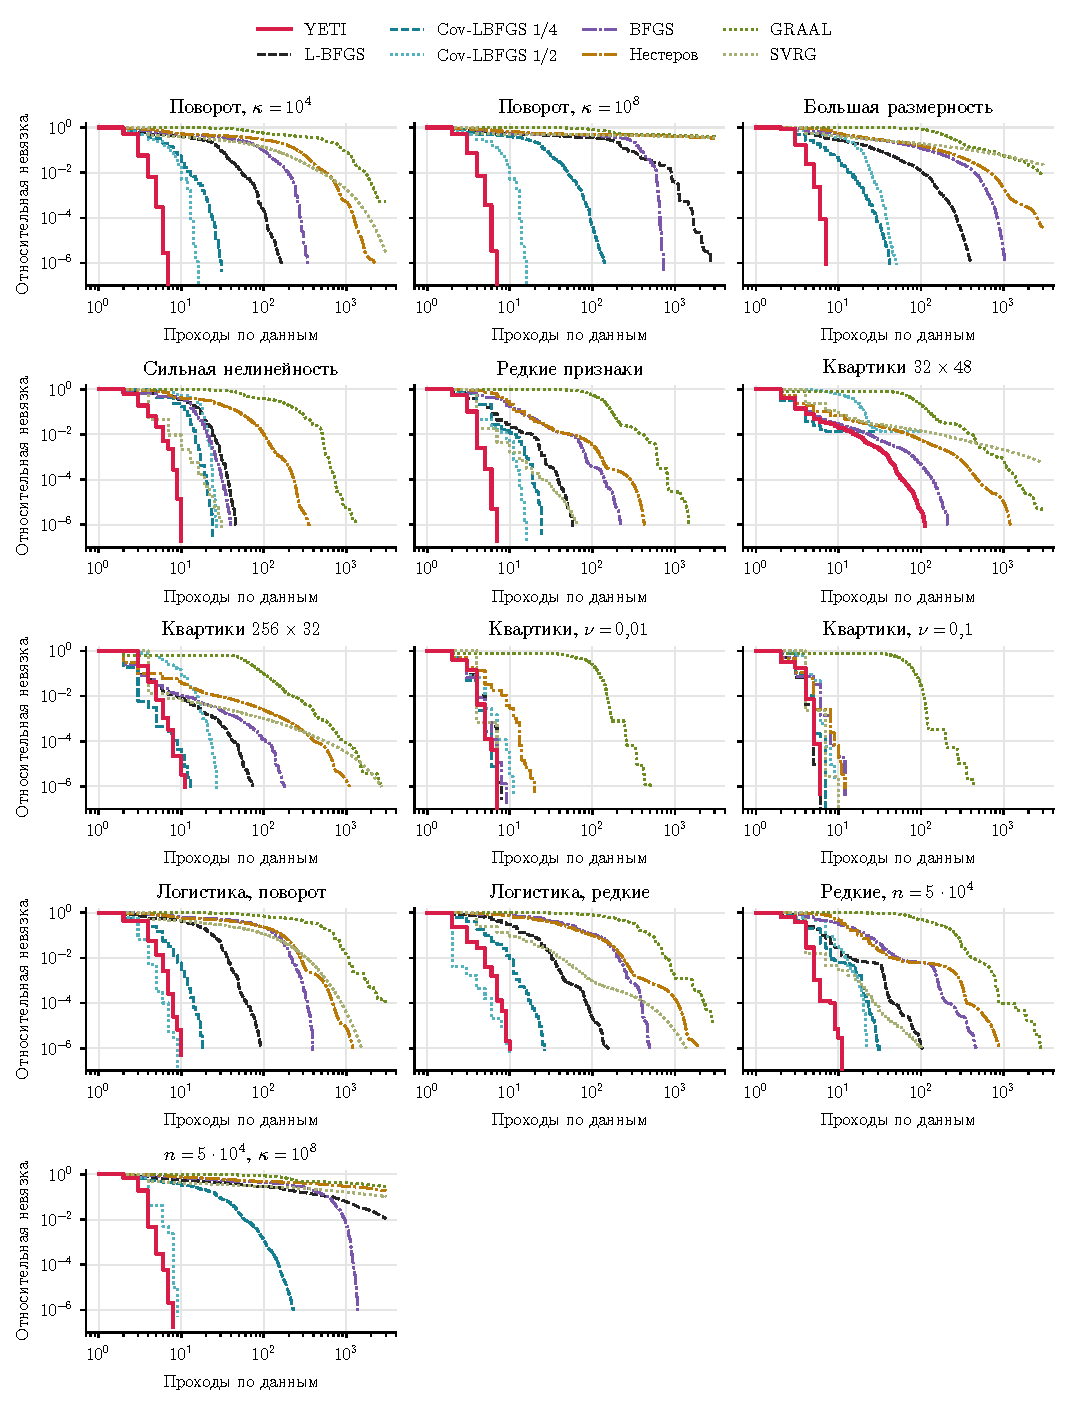
\includegraphics[width=\linewidth]{figures/families.pdf}
 \caption{Наименьшая достигнутая к данному моменту относительная невязка на первом экземпляре
 каждого семейства (обе шкалы логарифмические; YETI выделен красным; $\kappa$ --- число
 обусловленности ковариационной матрицы признаков).}
 \label{fig:exp-families}
\end{figure}

На цепочках YETI работает примерно так же, как L-BFGS. На пяти
пуассоновских задачах он достигает относительной точности $10^{-4}$
за 4--9 проходов; на freMTPL2freq методу SAGA требуется меньше проходов:
5 против 7 (табл.~\ref{tab:exp-chains}, \ref{tab:exp-glm}).

\paragraph{Остановка.}\label{sec:exp-certificate}
Критерий остановки по истории запросов~\eqref{eq:history-stop} не использует
эталонное значение. При $\varepsilon=10^{-6}\widehat\Delta$ он срабатывает
на всех 65 задачах, и все возвращённые точки удовлетворяют допуску
относительно эталона. Медиана числа проходов до остановки равна 15,
максимум --- 273. Критерий может срабатывать позже, чем допуск фактически
достигнут (рис.~\ref{fig:exp-certificate}).

\paragraph{Тестовые задачи.}
Цепочки S и X --- численные варианты трудных семейств из
раздела~\ref{sec:lower-origin}. Пуассоновские модели --- это синтетические задачи
и задачи на данных Bike Sharing и freMTPL2freq. Тринадцать семейств,
из которых составлены 65 задач (их названия указаны на рис.~\ref{fig:exp-families}
и в табл.~\ref{tab:exp-series}), устроены следующим образом.
\begin{itemize}
\item \emph{Поворот, $\kappa$}: пуассоновская регрессия, в которой
ковариационная матрица признаков имеет число обусловленности
$\kappa\in\{10^4,10^8\}$ и не диагональна в исходном базисе (её собственные
векторы повёрнуты относительно координатных осей).
\item \emph{Большая размерность}: пуассоновская регрессия с большим числом
признаков: $n=600$, $d=160$, $\kappa=10^4$.
\item \emph{Сильная нелинейность}: пуассоновская регрессия, в которой
истинный вектор параметров, по которому генерируются отклики, в три раза
длиннее, чем в остальных пуассоновских семействах; это увеличивает разброс
линейных предикторов $a_i^{\mathsf T}x$ и значений экспоненты.
\item \emph{Редкие признаки} и \emph{Редкие, $n=5\cdot10^4$}: пуассоновская
регрессия с разреженными признаками; во втором семействе число слагаемых
равно $5\cdot10^4$.
\item \emph{$n=5\cdot10^4$, $\kappa=10^8$}: плохо обусловленная
пуассоновская регрессия с $5\cdot10^4$ слагаемыми.
\item \emph{Квартики}: суммы квартических функций
$f_i(x)=\frac12(x-c_i)^{\mathsf T}H_i(x-c_i)+\frac\nu4\norm{x-c_i}^4$,
где $H_i\succ0$, а $c_i$ --- случайные центры. В названиях семейств
$32\times48$ и $256\times32$ указаны число слагаемых $n$ и размерность $d$;
$\nu$ --- вес слагаемого четвёртой степени (в этих двух семействах
$\nu=10^{-6}$).
\item \emph{Логистика, поворот} и \emph{Логистика, редкие}: регуляризованная
логистическая регрессия с повёрнутыми и с разреженными признаками
соответственно.
\end{itemize}
\FloatBarrier

\section{Нижняя оценка для произвольных запросов}\label{sec:lower}

Оценим снизу число запросов, необходимое любому методу,
который решает все задачи рассматриваемого класса.

\subsection{Происхождение четырёх слагаемых}\label{sec:lower-origin}

Нижнюю оценку докажем отдельно для каждого из четырёх слагаемых. Обозначим
\begin{equation}\label{eq:lower-four-terms}
 \begin{gathered}
 B_n=n,\\
 B_S=\sqrt{\frac{nL_0R^2}{\varepsilon}},\\
 B_Q=n(L_1R)^{2/3},\\
 B_X=\sqrt{\frac{nL_1^2R^2\delta}{\varepsilon}+n(L_1R)^2}.
 \end{gathered}
\end{equation}
Поскольку $\sqrt{a^2+b^2}\sim a+b$ при $a,b\ge0$, имеем
$T_0\sim B_n+B_S+B_X+B_Q$.

\begin{center}
\small
\renewcommand{\arraystretch}{1.18}
\begin{tabularx}{\linewidth}{@{}lYY@{}}
\toprule
Член & Что затрудняет решение & Трудное семейство\\
\midrule
$B_n$ & Поиск информативной компоненты & Скрытая пара функций\\
$B_S$ & Последовательное раскрытие гладких цепочек & Независимые цепочки S\\
$B_X$ & Неоднородность компонент при обобщённой гладкости & Экспоненциальные цепочки X\\
$B_Q$ & Повторный поиск компоненты для следующего шага & Цепочка Q со скрытым размещением звеньев\\
\bottomrule
\end{tabularx}
\end{center}

Для каждого слагаемого построим своё семейство задач.
Поскольку метод должен решать задачи всех четырёх семейств,
его сложность не меньше максимума полученных оценок.
Ниже зависимости обсуждаются с точностью до числовых и логарифмических
множителей. Точные условия конструкций приведены в приложении;
если отдельная конструкция неприменима, соответствующий член
оценивается через остальные.

\paragraph{Поиск информативной компоненты: $B_n=n$.}
Среди $n$ компонент случайно выбираются две ненулевые, остальные
равны нулю. До первого
обращения к одной из них алгоритм получает только нулевые ответы.
Эти ответы не позволяют различить две задачи с точками минимума по разные
стороны от начальной точки. Чтобы ожидаемая ошибка была мала,
нужно с достаточной вероятностью найти скрытую пару функций, а для этого
требуется порядка $n$ обращений к оракулу
(лемма~\ref{lem:lower-pair}).

\paragraph{Независимые гладкие цепочки: $B_S$.}
В каждую компоненту помещается своя цепочка координат. Под цепочкой
понимается функция, у которой очередная координата влияет на ответ
оракула только после достаточного продвижения по предыдущим
координатам. В идеализированной модели один запрос раскрывает не более
одного нового звена одной цепочки. Как это свойство переносится на
произвольные запросы, объяснено ниже.

В семействе S число звеньев одной цепочки имеет порядок
$\sqrt{L_0R^2/(n\varepsilon)}$. Чтобы достичь точности $\varepsilon$, нужно
раскрыть достаточную долю от общего числа звеньев всех цепочек. Поэтому
число запросов имеет порядок
\[
 n\sqrt{\frac{L_0R^2}{n\varepsilon}}
 =\sqrt{\frac{nL_0R^2}{\varepsilon}}=B_S.
\]
Задачи этого семейства гладкие: $\|\nabla^2f_i\|\le L_0$
(лемма~\ref{lem:lower-S}). Если условия построения цепочки не выполнены, то
$B_S\lesssim B_n$ и достаточно оценки для $B_n$.

\paragraph{Экспоненциальные цепочки: $B_X$.}
При обобщённой гладкости кривизна компоненты может расти вместе
с её градиентом. Даже в точке минимума среднего, где
$\nabla f(x^\ast)=0$, отдельные градиенты $\nabla f_i(x^\ast)$
могут быть ненулевыми и компенсировать друг друга. Поэтому малость нормы градиента среднего не влечёт
малости констант гладкости компонент.
Параметр $\delta$ ограничивает расхождение между минимумом среднего
и средним значением инфимумов компонент.

В семействе X цепочки входят в показатели
экспонент у компонент, объединённых в пары. Конструкция сохраняет последовательное
раскрытие звеньев и задаёт неоднородность, равную $\delta$.
Оценка для этого семейства вместе с оценкой для скрытой пары функций даёт $B_X$
(леммы~\ref{lem:lower-X} и~\ref{lem:lower-pair}). Поскольку
$B_X=\sqrt n\,L_1R\sqrt{1+\delta/\varepsilon}$, имеем
\[
  B_X\sim\sqrt n\,L_1R\max\left\{1,\sqrt{\frac\delta\varepsilon}\right\}.
\]

\paragraph{Поиск следующего звена: $B_Q$.}
В семействе Q используется одна цепочка, но её звенья случайно
размещены по парам компонент. После раскрытия очередной координаты
недостаточно знать, в каком направлении продолжать: нужно ещё
найти пару, в которой находится следующее звено. Компонента, которая уже
была запрошена, может стать информативной лишь на следующем уровне
цепочки, поэтому однократное вычисление всех компонент не избавляет
от этих поисков.

При условиях леммы~\ref{lem:lower-Q} длина цепочки имеет порядок
$(L_1R)^{2/3}$, а поиск пары на очередном уровне требует порядка $n$
запросов в среднем. Отсюда с точностью до логарифмических множителей
\[
 \underbrace{(L_1R)^{2/3}}_{\text{число уровней}}
 \;\underbrace{n}_{\text{поиск на уровне}}
 =B_Q.
\]
Показатель $2/3$ объясняется выбором длины цепочки $T$.
В точке минимума её $T$ активных координат равны $R/\sqrt T$, так
что норма этой точки равна $R$. Оценка невязки через число раскрытых
звеньев~\eqref{eq:lower-Q-gap} показывает, что для достижения точности
нужно пройти порядка $L_1R/\sqrt T$ уровней (с точностью до
логарифмических множителей), а всего уровней $T$. Длина цепочки
выбирается так, чтобы величины $T$ и $L_1R/\sqrt T$ совпадали
с точностью до абсолютных постоянных. Из равенства $T=L_1R/\sqrt T$
получаем $T^{3/2}=L_1R$, то есть $T=(L_1R)^{2/3}$; в
лемме~\ref{lem:lower-Q} выбрано целое $T$ этого порядка.
Точные условия этого выбора учитывают также начальную
невязку и неоднородность. Число обращений к оракулу, необходимое
для поиска следующего звена, оценивается в леммах~\ref{lem:lower-search}
и~\ref{lem:lower-revelations}.

\subsection{Нижняя оценка}

Пусть выполнены предположения~\ref{asm:components}--\ref{asm:accuracy}.
Число $N_0$ задано в~\eqref{eq:complexity-parameters}.

\proofdown{thm:lower}
\begin{theorem}\label{thm:lower}
Для оракула, возвращающего $(f_i(x),\nabla f_i(x))$, выполнено
\[
 \mathcal T^\ast\gtrsim\frac{T_0}{\log^2N_0}.
\]
\end{theorem}

Правая часть не зависит от $\Delta$ при $\Delta\ge2\varepsilon$.
Оценка относится к наихудшей задаче класса в произвольной размерности.
Метод может быть рандомизированным и выбирать точки запросов во всём
пространстве, а не только в линейной оболочке ранее полученных градиентов.

Вместе с верхней оценкой для YETI (теорема~\ref{thm:cheap-upper})
эта теорема показывает, что в данной постановке показатели степеней
при $n$, $L_0$, $L_1$, $R$, $\delta$ и $\varepsilon$ улучшить нельзя
(с точностью до логарифмических множителей). Логарифмический разрыв между верхней и нижней оценками
здесь не устраняется. Предположение~\ref{asm:accuracy} существенно для области
применимости результата: эту нижнюю оценку нельзя автоматически
переносить, например, на подкласс с $\delta=0$. Равенство $\delta=0$ означает,
что точка $x^\ast$ минимизирует каждую компоненту, то есть у всех $f_i$ есть
общая точка минимума. Для этого случая оценки сходимости стохастических
методов $(L_0,L_1)$-SGD и SGD-PS получены в работе
\citet[раздел~7]{gorbunov2024methods}.

\subsection{Доказательство нижней оценки}

\begin{proof}[Схема доказательства теоремы~\ref{thm:lower}]
Задача со скрытой парой функций даёт оценку для $B_n$.
Семейство S даёт оценку для $B_S$, а если его условия
нарушены, используется $B_S\lesssim B_n$.
Семейство X вместе со скрытой парой функций даёт оценку для $B_X$
с точностью до логарифмического множителя. Семейство Q даёт оценку для
$B_Q$. Когда условия~\eqref{eq:lower-Q-regime} не выполнены,
этот член оценивается через уже полученные оценки.

Следовательно,
\[
 T_0\sim\max\{B_n,B_S,B_X,B_Q\}
 \lesssim\mathcal T^\ast\log^2N_0.
\]
Леммы~\ref{lem:lower-finite}--\ref{lem:lower-revelations}
позволяют применить эти оценки к произвольным рандомизированным
методам. Разбор всех режимов параметров приведён
в приложении~\ref{app:lower-constants}.
\end{proof}

\section{Заключение}\label{sec:conclusion}
Для минимизации суммы выпуклых $(L_0,L_1)$-гладких функций метод YETI
достигает верхней оценки $O(T_0\log^2N)$, а для любого корректного метода
доказана нижняя оценка $\Omega(T_0/\log^2N_0)$. Если $\Delta/\varepsilon\le N_0^c$
при некотором фиксированном $c\ge1$, то эти оценки совпадают с точностью
до степеней $\log N_0$. Без ограничения на рост начальной невязки $\Delta$
оптимальность верхней оценки не установлена.

На 65 задачах при относительной точности $10^{-4}$ испытанный вариант YETI
занял первое место (в том числе разделив его с другими методами)
в 46 случаях, а его критерий остановки по истории запросов сработал
на всех 65 задачах. Основной выигрыш в этих опытах даёт эвристика
(приложение~\ref{app:experiments}). Однако её матричные операции могут
быть дорогими, поэтому выигрыш в числе запросов не обязательно означает
такой же выигрыш во времени.

\subsection{Открытые вопросы}\label{sec:open-questions}
\begin{enumerate}
\item \emph{Большая начальная невязка.}
Какова оптимальная зависимость сложности от $\Delta$?
Если $\log(\Delta/\varepsilon)$ имеет порядок $L_1R$, то полученные верхняя
и нижняя оценки могут различаться полиномиально по $L_1R$. Нужно либо
улучшить верхнюю оценку, либо доказать нижнюю оценку, учитывающую $\Delta$.
При умеренных $\Delta$ остаётся устранить логарифмический разрыв.

\item \emph{Индивидуальные константы гладкости.}
Можно ли получить более точную оценку сложности для заданного набора
$(L_{0,i},L_{1,i})$, не заменяя все $L_{1,i}$ их максимумом?
Неравномерный выбор компонент уже позволяет обойтись средним
значением $L_{0,i}$ (приложение~\ref{app:variants}). Чтобы улучшить общую
оценку, нужно учесть связь между $L_{1,i}$ и невязками отдельных слагаемых
и построить соответствующую нижнюю оценку: наша нижняя оценка получена
на подклассе с одинаковыми $L_{0,i}$.

\item \emph{Ограничения и неевклидова геометрия.}
Как перенести результат на минимизацию по выпуклому множеству
и на методы с расстоянием Брэгмана? Зеркальный спуск при обобщённой
гладкости изучен в работе~\citet{yu2026mirror}. Здесь дополнительно
потребуются анализ уменьшения дисперсии, замена евклидова потенциала
и оценка числа отсечений.

\item \emph{Негладкие слагаемые.}
Можно ли получить аналогичные двусторонние оценки для конечных сумм,
у которых нормы субградиентов ограничены через невязку?
Такая негладкая стохастическая постановка рассматривается в работе
\citet{kovalev2026nonsmooth}. Для конечной суммы нужно отдельно определить
модель оракула и выяснить, какой выигрыш даёт уменьшение дисперсии.

\item \emph{Методы второго и более высоких порядков.}
Можно ли совместить уменьшение дисперсии для конечных сумм
\citep{tsedenov2026second} с ускорением при обобщённой гладкости
гессиана \citep{agafonov2026inexact}? Для этого нужны оценки ошибок
стохастических производных и новый локальный решатель. Условия на старшие
производные не следуют из предположения~\ref{asm:smoothness}.

\item \emph{Двойственная задача.}
Можно ли интерпретировать YETI как покоординатный метод для двойственной
задачи и связать его со схемой из работы \citet{podlipnova2026sparse}?
Помимо преобразования задачи, потребуется сопоставить доступные оракулы
и стоимость одного шага: запрос компоненты $f_i$ и запрос координаты
двойственного градиента в общем случае не эквивалентны.
\end{enumerate}

Отдельно остаётся найти сложность вне области действия
предположения~\ref{asm:accuracy}, в частности при $\delta=0$.
Этот вопрос касается неоднородности слагаемых и не совпадает
с вопросом о большой начальной невязке $\Delta$.

% Литература сразу после основной части, мельче основного текста.
\begingroup
\selectlanguage{english}
\renewcommand{\refname}{Литература}
\renewcommand{\bibfont}{\small}
\bibliographystyle{plainnat}
\bibliography{refs}
\endgroup
% Приложения с новой страницы и мельче основного текста,
% чтобы длинные выкладки помещались в строку.
\clearpage
\appendix
\begingroup
\small
\section{Аналитические свойства класса}\label{sec:analytic-tools}

Вспомогательные леммы сформулированы для произвольной функции $\varphi$.
К компонентам $f_i$ они применяются в силу предположений~\ref{asm:components}
и~\ref{asm:smoothness} с константой $L_{0,i}$ вместо $L_0$.

\subsection{Локальная гладкость}

См. также \citet[лемма~A.1]{rudomanov2026everest}
и \citet[лемма~2.5]{vankov2025optimizing}.

\begin{lemma}[рост градиента вдоль отрезка]\label{lem:local-transfer}
Пусть $\varphi\in C^2(\mathbb R^d)$ и
$\norm{\nabla^2\varphi(x)}\le L_0+L_1\norm{\nabla\varphi(x)}$
для всех $x$. Тогда для любых $x,y$ выполняется
\begin{equation}\label{eq:local-transfer}
 L_0+L_1\norm{\nabla\varphi(x)}
 \le e^{L_1\norm{x-y}}
       \bigl(L_0+L_1\norm{\nabla\varphi(y)}\bigr).
\end{equation}
В частности, на шаре $B(y,r)$ градиент $\varphi$ липшицев с константой
$e^{L_1r}(L_0+L_1\norm{\nabla\varphi(y)})$.
\end{lemma}

\begin{proof}
По формуле Ньютона--Лейбница
\[
 \nabla\varphi(y+t(x-y))-\nabla\varphi(y)
 =\int_0^t\nabla^2\varphi(y+u(x-y))(x-y)\,du.
\]
Взяв норму и применив условие на гессиан, для $t\in[0,1]$ получаем
\[
 L_0+L_1\norm{\nabla\varphi(y+t(x-y))}
 \le L_0+L_1\norm{\nabla\varphi(y)}
 +L_1\norm{x-y}\int_0^t\bigl(L_0+L_1\norm{\nabla\varphi(y+u(x-y))}\bigr)\,du.
\]
По неравенству Гронуолла
\[
 L_0+L_1\norm{\nabla\varphi(y+t(x-y))}
 \le e^{L_1\norm{x-y}t}\bigl(L_0+L_1\norm{\nabla\varphi(y)}\bigr).
\]
При $t=1$ получаем первое утверждение. Для $x\in B(y,r)$ оно даёт оценку
нормы гессиана на всём шаре, а интегрирование гессиана по отрезкам
внутри выпуклого шара доказывает липшицевость градиента.
\end{proof}

\citep[Теорема Байона--Хаддада,][]{bauschke2010}

\begin{lemma}[кокоэрцитивность на выпуклой области]\label{lem:local-cocoercivity}
Пусть $\varphi$ выпукла и дважды непрерывно дифференцируема
в окрестности выпуклого множества $\mathcal D$. Если
$\norm{\nabla^2\varphi}\le L$ на $\mathcal D$, где $L>0$, то для всех
$x,z\in\mathcal D$
\[
 \norm{\nabla\varphi(x)-\nabla\varphi(z)}^2
 \le L\ip{\nabla\varphi(x)-\nabla\varphi(z)}{x-z}.
\]
\end{lemma}

\begin{proof}
Средний гессиан
\[
 H=\int_0^1\nabla^2\varphi(z+t(x-z))\,dt
\]
удовлетворяет $0\preceq H\preceq LI$ по выпуклости, поэтому
$H^2\preceq LH$ и
\[
 \norm{\nabla\varphi(x)-\nabla\varphi(z)}^2
 =\ip{x-z}{H^2(x-z)}
 \le L\ip{x-z}{H(x-z)}
 =L\ip{\nabla\varphi(x)-\nabla\varphi(z)}{x-z}.
\]
\end{proof}

\begin{lemma}[оценка разности градиентов]\label{lem:local-bregman}
Пусть $\varphi$ выпукла, $\varphi\in C^2(\mathbb R^d)$ и
$\norm{\nabla^2\varphi}\le L$ на $B(y,3r)$, где $L>0$.
Тогда для $x,w\in B(y,r)$ выполнено
\[
 \norm{\nabla\varphi(x)-\nabla\varphi(w)}^2
 \le2L\bigl(\varphi(x)-\varphi(w)
                     -\ip{\nabla\varphi(w)}{x-w}\bigr).
\]
\end{lemma}

\begin{proof}
Так как градиент функции $\varphi$ является $L$-липшицевым на $B(y,r)$
и $x,w\in B(y,r)$, имеем
\[
 \norm{\nabla\varphi(x)-\nabla\varphi(w)}\le L\norm{x-w}\le2Lr.
\]
Поэтому точка
\[
 q=x-\frac1L\bigl(\nabla\varphi(x)-\nabla\varphi(w)\bigr)
\]
лежит в $B(y,3r)$, а значит, и весь отрезок $[x,q]$ содержится в $B(y,3r)$.
Функция
\[
 z\mapsto\varphi(z)-\varphi(w)-\ip{\nabla\varphi(w)}{z-w}
\]
выпукла, неотрицательна во всём пространстве и имеет на $B(y,3r)$
$L$-липшицев градиент $\nabla\varphi(z)-\nabla\varphi(w)$.
Квадратичная оценка сверху на отрезке $[x,q]$ даёт
\begin{align*}
 0&\le\varphi(q)-\varphi(w)-\ip{\nabla\varphi(w)}{q-w}
 \\&\le\varphi(x)-\varphi(w)-\ip{\nabla\varphi(w)}{x-w}
   +\ip{\nabla\varphi(x)-\nabla\varphi(w)}{q-x}+\frac L2\norm{q-x}^2
 \\&=\varphi(x)-\varphi(w)-\ip{\nabla\varphi(w)}{x-w}
   -\frac1{2L}\norm{\nabla\varphi(x)-\nabla\varphi(w)}^2.
\end{align*}
Остаётся перенести последнее слагаемое в левую часть.
\end{proof}

\subsection{Оценка нормы градиента через невязку}

Ср. \citet{li2023generalized} и \citet[лемма~3.4]{yu2026mirror}.

\begin{lemma}[интегральная оценка нормы градиента]\label{lem:self-bound}
Пусть $\varphi$ выпукла, ограничена снизу, принадлежит
$C^2(\mathbb R^d)$ и удовлетворяет условию леммы~\ref{lem:local-transfer}.
Тогда для любого $x$
\begin{equation}\label{eq:integral-self-bound}
 \begin{gathered}
 \int_0^{\norm{\nabla\varphi(x)}}\frac{t}{L_0+L_1t}\,dt
 \le\varphi(x)-\inf\varphi,\\
 \norm{\nabla\varphi(x)}
 \le L_1\bigl(\varphi(x)-\inf\varphi\bigr)
 +\sqrt{2L_0\bigl(\varphi(x)-\inf\varphi\bigr)}.
 \end{gathered}
\end{equation}
При $L_0=0$ подынтегральная функция доопределяется в нуле по непрерывности.
Достижимость инфимума не предполагается.
\end{lemma}

\begin{proof}
При $\nabla\varphi(x)=0$ утверждение очевидно. Иначе выберем $h>0$ так, чтобы
\[
 \begin{gathered}
 L_1h\norm{\nabla\varphi(x)}\le\tfrac12,\\
 h\bigl(L_0+L_1\norm{\nabla\varphi(x)}\bigr)\le\tfrac12,
 \end{gathered}
\]
и рассмотрим градиентный спуск из точки $x_0=x$:
\[
 x_{j+1}=x_j-h\nabla\varphi(x_j).
\]

\begin{itemize}
\item Норма градиента не возрастает. Пусть
$\norm{\nabla\varphi(x_j)}\le\norm{\nabla\varphi(x)}$. Отрезок
$[x_j,x_{j+1}]$ имеет длину $h\norm{\nabla\varphi(x_j)}$, поэтому
по лемме~\ref{lem:local-transfer} норма гессиана на нём не превосходит
\begin{equation}\label{eq:self-bound-step-curvature}
 e^{L_1h\norm{\nabla\varphi(x_j)}}
 \bigl(L_0+L_1\norm{\nabla\varphi(x_j)}\bigr)
 \le2\bigl(L_0+L_1\norm{\nabla\varphi(x)}\bigr)
 \le\frac1h.
\end{equation}
Значит, средний гессиан $H_j$ на этом отрезке удовлетворяет
$0\preceq hH_j\preceq I$, и
\[
 \begin{gathered}
 \nabla\varphi(x_{j+1})=(I-hH_j)\nabla\varphi(x_j),\\
 \norm{\nabla\varphi(x_{j+1})}\by{\le}{(a)}\norm{\nabla\varphi(x_j)}.
 \end{gathered}
\]
Здесь (a) следует из $0\preceq I-hH_j\preceq I$.
По индукции эти оценки верны для всех $j$.

\item Оценим две телескопические суммы. Квадратичная оценка сверху
вместе с оценкой кривизны~\eqref{eq:self-bound-step-curvature} даёт
\[
 \varphi(x_j)-\varphi(x_{j+1}) \ge h\norm{\nabla\varphi(x_j)}^2
 -\frac{h^2}{2}e^{L_1h\norm{\nabla\varphi(x_j)}}
 \bigl(L_0+L_1\norm{\nabla\varphi(x_j)}\bigr)\norm{\nabla\varphi(x_j)}^2 \ge\frac h2\norm{\nabla\varphi(x_j)}^2.
\]
Подынтегральная функция $t/(L_0+L_1t)$ не убывает, а
\[
 \norm{\nabla\varphi(x_j)}-\norm{\nabla\varphi(x_{j+1})}
 \le\norm{hH_j\nabla\varphi(x_j)}.
\]
Поэтому
\[
 \int_{\norm{\nabla\varphi(x_{j+1})}}^{\norm{\nabla\varphi(x_j)}}
 \frac{t\,dt}{L_0+L_1t} \le\frac{\norm{\nabla\varphi(x_j)}}{L_0+L_1\norm{\nabla\varphi(x_j)}}
 \norm{hH_j\nabla\varphi(x_j)} \by{\le}{(a)}
 he^{L_1h\norm{\nabla\varphi(x_j)}}\norm{\nabla\varphi(x_j)}^2.
\]
Здесь (a) следует из оценки~\eqref{eq:self-bound-step-curvature}
для $\norm{H_j}$. Так как $e^s-1\le2s$ и $e^s\le2$ при $0\le s\le1/2$,
из оценки убывания функции и последней оценки интеграла получаем
\[
 \int_{\norm{\nabla\varphi(x_{j+1})}}^{\norm{\nabla\varphi(x_j)}}
 \frac{t\,dt}{L_0+L_1t}
 \le\varphi(x_j)-\varphi(x_{j+1})
 +h^2\bigl(L_0+3L_1\norm{\nabla\varphi(x)}\bigr)\norm{\nabla\varphi(x_j)}^2.
\]
Суммируя неравенство
\[
 \varphi(x_i)-\varphi(x_{i+1})\ge\frac h2\norm{\nabla\varphi(x_i)}^2
\]
по $i=0,\ldots,m-1$, получаем
\[
 h\sum_{i<m}\norm{\nabla\varphi(x_i)}^2\le2\bigl(\varphi(x)-\inf\varphi\bigr).
\]
Суммируя оценку разности интегралов по $i=0,\ldots,j-1$, где $0\le j<m$,
и используя полученную оценку суммы квадратов норм градиентов, получаем
\[
 \int_0^{\norm{\nabla\varphi(x)}}\frac{t\,dt}{L_0+L_1t}
 \le\bigl(\varphi(x)-\inf\varphi\bigr)
 \Bigl(1+2h\bigl(L_0+3L_1\norm{\nabla\varphi(x)}\bigr)\Bigr)
 +\int_0^{\norm{\nabla\varphi(x_j)}}\frac{t\,dt}{L_0+L_1t}.
\]
Возьмём $m=\lceil h^{-2}\rceil$ и индекс $j<m$ с наименьшей нормой
$\norm{\nabla\varphi(x_j)}$. Тогда
\[
 \norm{\nabla\varphi(x_j)}^2
 \le\frac{2(\varphi(x)-\inf\varphi)}{mh}\to0
 \quad\text{при }h\downarrow0.
\]
Последний интеграл не превосходит $\norm{\nabla\varphi(x_j)}/L_1$,
поэтому, переходя к пределу, получаем первое
неравенство~\eqref{eq:integral-self-bound}.

\item При $L_0=0$ интеграл равен $\norm{\nabla\varphi(x)}/L_1$, что сразу
даёт второе неравенство. При $L_0>0$ после замены $t=L_0s/L_1$
интегральная оценка принимает вид
\[
 \frac{L_1\norm{\nabla\varphi(x)}}{L_0}
 -\log\Bigl(1+\frac{L_1\norm{\nabla\varphi(x)}}{L_0}\Bigr)
 \le\frac{L_1^2(\varphi(x)-\inf\varphi)}{L_0}.
\]
Функция $s\mapsto s-\log(1+s)$ возрастает при $s\ge0$. Для
$v\ge0$ из разложения экспоненты в ряд следует $e^{\sqrt{2v}}\ge1+\sqrt{2v}+v$, поэтому
\[
 (v+\sqrt{2v})-\log(1+v+\sqrt{2v})\ge v.
\]
Применив это неравенство при $v=L_1^2(\varphi(x)-\inf\varphi)/L_0$, получаем
\[
 \frac{L_1\norm{\nabla\varphi(x)}}{L_0}
 \le\frac{L_1^2(\varphi(x)-\inf\varphi)}{L_0}
 +\sqrt{\frac{2L_1^2(\varphi(x)-\inf\varphi)}{L_0}},
\]
что и требовалось.
\end{itemize}
\end{proof}

\subsection{Оценка локальной кривизны суммы}\label{app:observed-curvature}

\begin{proof}[Доказательство леммы~\ref{lem:observed-curvature}\proofup{lem:observed-curvature}]
Для среднего неотрицательных величин $f_i(y)-\inf f_i$ имеем
\[
 \frac1n\sum_i\bigl(f_i(y)-\inf f_i\bigr)
 =f(y)-f^\ast+f^\ast-\frac1n\sum_i\inf f_i
 \by{\le}{\text{\ref{asm:heterogeneity}}}\delta+f(y)-f^\ast.
\]
По лемме~\ref{lem:self-bound}, применимой в силу
предположений~\ref{asm:components} и~\ref{asm:smoothness},
\begin{align*}
 &\frac1n\sum_i\norm{\nabla f_i(y)}\le\frac{L_1}n\sum_i\bigl(f_i(y)-\inf f_i\bigr)
 +\frac1n\sum_i\sqrt{2L_{0,i}\bigl(f_i(y)-\inf f_i\bigr)}
 \\&\qquad\by{\le}{(a)}
 L_1\bigl(\delta+f(y)-f^\ast\bigr)+\sqrt{2L_0\bigl(\delta+f(y)-f^\ast\bigr)},
 \\
 &\ell(y)\le L_0+L_1^2\bigl(\delta+f(y)-f^\ast\bigr)
 +L_1\sqrt{2L_0\bigl(\delta+f(y)-f^\ast\bigr)}
 \\&\qquad\by{\le}{(b)}
 \tfrac32L_0+2L_1^2\bigl(\delta+f(y)-f^\ast\bigr).
\end{align*}
В (a) использованы неравенство Коши--Буняковского--Шварца
и ограничение на среднее значение $L_{0,i}$ из предположения~\ref{asm:smoothness};
(b) следует из $2ab\le a^2+b^2$.
Неравенство треугольника даёт обе оценки для $\norm{\nabla f(y)}$.
Остальные утверждения получаются суммированием оценок
леммы~\ref{lem:local-transfer} с учётом предположения~\ref{asm:smoothness}.
\end{proof}

\Needspace{10\baselineskip}
\subsection{Вырожденный класс}\label{app:degenerate}

\begin{proposition}\label{prop:degenerate-class}
При предположениях~\ref{asm:components}--\ref{asm:minimizer}
и~\ref{asm:heterogeneity}, если $L_0=\delta=0$, то все компоненты постоянны.
Следовательно, минимаксная оракульная сложность такого класса равна нулю.
\end{proposition}

\begin{proof}
В силу предположения~\ref{asm:smoothness} из $L_0=0$ следует
$L_{0,i}=0$. В точке $x^\ast$ из предположения~\ref{asm:minimizer} имеем
\[
 0\le\frac1n\sum_i\bigl(f_i(x^\ast)-\inf f_i\bigr)
 =f^\ast-\frac1n\sum_i\inf f_i\by{\le}{\text{\ref{asm:heterogeneity}}}\delta=0.
\]
Значит, каждое слагаемое равно нулю, откуда $\nabla f_i(x^\ast)=0$.
Лемма~\ref{lem:local-transfer} при $L_{0,i}=0$ даёт
\[
 \norm{\nabla f_i(x)}\le e^{L_1\norm{x-x^\ast}}
 \norm{\nabla f_i(x^\ast)}=0
\]
для любого $x$. Следовательно, все компоненты постоянны, и ответ $0$
можно выдать без единого запроса к оракулу.
\end{proof}


\section{Доказательства утверждений о методе YETI}\label{app:cheap-proofs}

\subsection{Нижние оценки по истории}\label{app:history-proofs}

\begin{proof}[Доказательство леммы~\ref{lem:history-small-gradient}\proofup{lem:history-small-gradient}]
Выберем точку $w\in B(0,R)$, минимизирующую линейную функцию
$u\mapsto\ip{\nabla f(z)}u$. По определению нормального конуса
$\ip{v_z}{w-z}\le0$. Поэтому
\[
 f(z)-\widetilde f(z)=\ip{\nabla f(z)}{z-w}
 \le\ip g{z-w}
 \by{\le}{(a)}\norm g\norm{z-w}
 \le2R\norm g,
\]
где (a) следует из неравенства Коши--Буняковского--Шварца.
После записи $z$ в историю имеем $f(w_{\rm best})\le f(z)$ и
$\widetilde f_{\rm best}\ge\widetilde f(z)$, что завершает доказательство.
\end{proof}

\subsection{Нижняя оценка по ответам отдельных компонент}\label{app:component-history}

Критерий остановки~\eqref{eq:history-stop} использует нижние
оценки~\eqref{eq:history-full-lower}, а каждая из них требует ответов
всех $n$ компонент в одной и той же точке. Эвристика в экспериментах
(приложение~\ref{app:experiments}) запрашивает отдельные компоненты
в разных точках. Покажем, что и такие ответы можно объединить в нижнюю
оценку $f^\ast$, не делая новых запросов. Этот подраздел нужен только
для экспериментов: в доказательстве оценки сложности YETI он
не используется.

Выберем для каждого индекса $i$ один из уже полученных ответов
этой компоненты; пусть он получен в точке $p_i$. Положим
\begin{equation}\label{eq:mixed-history-lower}
 \widetilde f_{\rm mix}
 =\frac1n\sum_{i=1}^n\bigl(f_i(p_i)-\ip{\nabla f_i(p_i)}{p_i}\bigr)
 -R\,\Bigl\|\frac1n\sum_{i=1}^n\nabla f_i(p_i)\Bigr\|.
\end{equation}
Если все точки $p_i$ совпадают с некоторой точкой $p$, то
$\widetilde f_{\rm mix}=\widetilde f(p)$, то есть~\eqref{eq:mixed-history-lower}
обобщает~\eqref{eq:history-full-lower}.

\begin{proposition}\label{prop:mixed-history}
Выполнено $\widetilde f_{\rm mix}\le f^\ast$. Поэтому величину
$\widetilde f_{\rm mix}$ можно учитывать в максимуме $\widetilde f_{\rm best}$
наравне с оценками~\eqref{eq:history-full-lower}. При замене одного
выбранного ответа пересчёт обеих сумм в~\eqref{eq:mixed-history-lower}
требует $O(d)$ арифметических операций и не требует новых запросов к оракулу.
\end{proposition}

\begin{proof}
В силу выпуклости компонент (предположение~\ref{asm:components})
для любого $w$
\[
 f(w)\ge\frac1n\sum_i\bigl(f_i(p_i)+\ip{\nabla f_i(p_i)}{w-p_i}\bigr).
\]
При $w=x^\ast$ предположение~\ref{asm:minimizer}
и неравенство Коши--Буняковского--Шварца дают
$f^\ast\ge\widetilde f_{\rm mix}$. Замена ответа с индексом $i$
меняет только одно слагаемое скалярной суммы и одно слагаемое
векторной суммы.
\end{proof}

Оценку~\eqref{eq:mixed-history-lower} можно вычислить только после того,
как для каждой компоненты получен хотя бы один ответ. Никаких условий
на точки $p_i$ или на порядок, в котором они получены, не требуется.
При последующих заменах ответов значение $\widetilde f_{\rm mix}$ может
уменьшиться, поэтому в $\widetilde f_{\rm best}$ хранится максимум всех
уже полученных нижних оценок. Для пересчёта $\widetilde f_{\rm mix}$
нужно хранить по одному выбранному ответу каждой компоненты; это
дополнительная память по сравнению с хранением только лучшей нижней
оценки и лучшей точки.

\Needspace{12\baselineskip}
\subsection{Локальный решатель}\label{app:local-proofs}

\begin{proof}[Доказательство леммы~\ref{lem:local-projection}\proofup{lem:local-projection}]
\leavevmode
\begin{itemize}
\item Для $\zeta\ge0$ рассмотрим точку
\[
 z_\zeta=\Pi_{B(0,R)}\Bigl(\frac{b+\zeta y}{1+\zeta}\Bigr).
\]
Она непрерывно зависит от $\zeta$ и стремится к $y$ при $\zeta\to\infty$.
Если $\norm{z_0-y}\le r$, достаточно взять $\zeta=0$. Иначе существует
$\zeta>0$, для которого $\norm{z_\zeta-y}=r$. Вид нормального конуса
к шару $B(0,R)$ даёт~\eqref{eq:two-ball-normal}. Для любого $t\in\mathcal K$ получаем
\[
 \ip{b-z}{t-z}
 =\xi\ip z{t-z}+\zeta\ip{z-y}{t-z}
 \by{\le}{(a)}0.
\]
Здесь (a) следует из того, что $\xi z$ и $\zeta(z-y)$ --- нормали
к шарам $B(0,R)$ и $B(y,r)$ в точке $z$.
Это неравенство характеризует проекцию на $\mathcal K$ и доказывает
утверждение, в том числе когда шары совпадают или один из них вложен в другой.
\item Неравенство \eqref{eq:local-bregman} следует из
леммы~\ref{lem:local-bregman} для $\varphi=P_i$ и $L=L_i$.
В шаре радиуса $3r$ лежит и вспомогательная точка из доказательства
этой леммы, поэтому к ней применима оценка гладкости.
Из выпуклости $P_i$, следующей из предположения~\ref{asm:components},
получаем неотрицательность
её отклонения от касательной. Кокоэрцитивность $P$ следует из
леммы~\ref{lem:local-cocoercivity}: на выпуклом шаре $B(y,r)$
средний гессиан $P$ лежит между $0$ и $\overline LI$.
Это локальный вариант классического свойства
кокоэрцитивности~\citep{baillon1977}.
\end{itemize}
\end{proof}

\Needspace{14\baselineskip}
Для локальной задачи и эпохи SVRG сохраняем обозначения $u$, $w$, $s$,
$h_s$, $M$ и $\overline L$ из раздела~\ref{sec:local-solver}.

\begin{lemma}[уменьшение функции Ляпунова за эпоху]\label{lem:svrg-contraction}
Положим
\begin{equation}\label{eq:svrg-potential}
 \Psi(w,s)=\norm{w-u}^2
 +4h_s^2\sum_{j=0}^{M-1}(1-h_s\lambda)^j\,
 \sum_{i=1}^n\frac{\norm{\nabla P_i(s)-\nabla P_i(u)}^2}{nL_i/\overline L}.
\end{equation}
Тогда условно относительно всей истории до начала эпохи
\begin{equation}\label{eq:svrg-contraction}
 \begin{gathered}
 \E\Psi(w^+,s^+)\le\tfrac12\Psi(w,s),\\
 \Psi(y,y)\le\left(1+\frac{2\overline L}{3\lambda}\right)\norm{y-u}^2.
 \end{gathered}
\end{equation}
\end{lemma}

\begin{proof}
\leavevmode
\begin{itemize}
\item Пусть случайный индекс $I$ принимает значение $i$ с вероятностью
$L_i/(n\overline L)$. Тогда
\[
 v_I-\nabla P(u)
 =\frac{\nabla P_I(x)-\nabla P_I(u)}{L_I/\overline L}
 +\Bigl(\nabla P(s)-\nabla P(u)
 -\frac{\nabla P_I(s)-\nabla P_I(u)}{L_I/\overline L}\Bigr).
\]
Второе слагаемое центрировано, а математическое ожидание квадрата его нормы
не превосходит суммы из~\eqref{eq:svrg-potential}. Для любой точки
$t\in B(y,r)$
\begin{equation}\label{eq:svrg-variance-bound}
 \sum_{i=1}^n\frac{\norm{\nabla P_i(t)-\nabla P_i(u)}^2}{nL_i/\overline L}
 \by{\le}{(a)}2\overline L\bigl(P(t)-P(u)-\ip{\nabla P(u)}{t-u}\bigr),
\end{equation}
где (a) следует из выбора вероятностей $L_i/(n\overline L)$, оценки~\eqref{eq:local-bregman}
и равенства $P=\frac1n\sum_iP_i$. Поэтому
\begin{align*}
 \E\norm{v_I-\nabla P(u)}^2&\by{\le}{(a)}2\sum_{i=1}^n\frac{\norm{\nabla P_i(x)-\nabla P_i(u)}^2}{nL_i/\overline L}+2\sum_{i=1}^n\frac{\norm{\nabla P_i(s)-\nabla P_i(u)}^2}{nL_i/\overline L}
 \\&\by{\le}{(b)}4\overline L\bigl(P(x)-P(u)-\ip{\nabla P(u)}{x-u}\bigr)
 +2\sum_{i=1}^n\frac{\norm{\nabla P_i(s)-\nabla P_i(u)}^2}{nL_i/\overline L}.
\end{align*}
Здесь (a) следует из неравенства
\[
 \norm{a+b}^2\le2\norm a^2+2\norm b^2,
\]
(b) --- из~\eqref{eq:svrg-variance-bound} при $t=x$.
\item Оптимальность $u$ означает
$u=\Pi_{\mathcal K}(u-h_s\nabla P(u))$. Поэтому
\begin{align*}
 \E\norm{x^+-u}^2&\by{\le}{(a)}
 \norm{x-u}^2-2h_s\ip{\nabla P(x)-\nabla P(u)}{x-u}
       +h_s^2\E\norm{v_I-\nabla P(u)}^2
 \\&\by{\le}{(b)}
 (1-h_s\lambda)\norm{x-u}^2
 -\frac43h_s\bigl(P(x)-P(u)-\ip{\nabla P(u)}{x-u}\bigr)
 \\&+2h_s^2\sum_{i=1}^n\frac{\norm{\nabla P_i(s)-\nabla P_i(u)}^2}{nL_i/\overline L}.
\end{align*}
Здесь (a) следует из нерастяжимости проекции и несмещённости $v_I$,
(b) --- из сильной выпуклости $P$, предыдущего пункта и равенства
$2h_s-4h_s^2\overline L=\frac43h_s$.
\item По \eqref{eq:svrg-parameters} имеем $0<h_s\lambda\le1/6$
и $h_s\lambda M\ge7/10$. Развернём полученное рекуррентное неравенство на всю эпоху.
Так как $8h_s^2\overline L=\frac43h_s$, слагаемые с остатками
линеаризации в точках $x_j$ сокращаются, и
\[
 \E\Psi(w^+,s^+) \by{\le}{(a)}
 (1-h_s\lambda)^M\norm{w-u}^2
 +2h_s^2\sum_{j=0}^{M-1}(1-h_s\lambda)^j\,\sum_{i=1}^n\frac{\norm{\nabla P_i(s)-\nabla P_i(u)}^2}{nL_i/\overline L} \by{\le}{(b)}\tfrac12\Psi(w,s).
\]
Здесь (a) следует из рекуррентного неравенства предыдущего пункта,
оценки~\eqref{eq:svrg-variance-bound} при $t=s^+$ и неравенства Йенсена
для выпуклой функции $t\mapsto P(t)-P(u)-\ip{\nabla P(u)}{t-u}$,
(b) --- из $(1-h_s\lambda)^M\le e^{-7/10}<1/2$.
Наконец, локальная гладкость даёт
\[
 P(y)-P(u)-\ip{\nabla P(u)}{y-u}\le\frac{\overline L}2\norm{y-u}^2,
\]
поэтому по~\eqref{eq:svrg-variance-bound} сумма
из~\eqref{eq:svrg-potential} при $s=y$ не превосходит $\overline L^2\norm{y-u}^2$.
Вместе с
\[
 \sum_{j=0}^{M-1}(1-h_s\lambda)^j\le\frac1{h_s\lambda}
\]
это даёт
\[
 \Psi(y,y)\le\left(1+\frac{4h_s\overline L^2}{\lambda}\right)\norm{y-u}^2
 =\left(1+\frac{2\overline L}{3\lambda}\right)\norm{y-u}^2.
\]
\end{itemize}
\end{proof}

\begin{proof}[Доказательство леммы~\ref{lem:local-certificate}\proofup{lem:local-certificate}]
\leavevmode
\begin{itemize}
\item По лемме~\ref{lem:local-projection} отображение
$I-\nabla P/\overline L$ нерастяжимо на $\mathcal K$. Сравнивая
проекции точек $w-\nabla P(w)/\overline L$ и $u-\nabla P(u)/\overline L$,
получаем первую оценку в \eqref{eq:sharp-residual}. Для второй оценки имеем
\begin{align*}
 \norm e^2&=\overline L^2\norm{w-z}^2
 -2\overline L\ip{\nabla P(w)-\nabla P(z)}{w-z}
 +\norm{\nabla P(w)-\nabla P(z)}^2
 \\&\by{\le}{(a)}\overline L\ip e{w-z}
 \by{\le}{(b)}\overline L\ip e{w-u}
 \by{\le}{(c)}\overline L\norm e\norm{w-u}.
\end{align*}
Здесь (a) следует из кокоэрцитивности $\nabla P$, (b) --- из неравенства
\[
 \ip e{z-u}\ge P(z)-P(u)\ge0,
\]
которое верно, поскольку $e\in\nabla P(z)+N_{\mathcal K}(z)$
по определению проекции, (c) --- из неравенства
Коши--Буняковского--Шварца.
\item Если $\norm{w-u}$ удовлетворяет условию леммы, то
\[
 \norm e\le\overline L\norm{w-u}
 \le\frac45\lambda\bigl(\norm{y-u}-\norm{w-u}\bigr)
 \le\frac45\lambda\norm{y-z}
 \le\frac45(\lambda+\beta)\norm{y-z}.
\]
Предпоследний переход следует из $\norm{z-u}\le\norm{w-u}$
и неравенства треугольника. Значит, выполнено второе
условие~\eqref{eq:certificate-test}.
Если $y=u$, то $\Psi(y,y)=0$, после первой эпохи почти наверное $w=u$,
и набор принимается. При $y\ne u$ после $j$ эпох
лемма~\ref{lem:svrg-contraction} и неравенство Маркова дают
\[
 \begin{aligned}
 \Pr(T_{\rm ep}>j)
 &\le\Pr\left(\norm{w_j-u}>\frac{4\lambda}{5\overline L+4\lambda}\norm{y-u}\right)\\
 &\le\left(1+\frac{5\overline L}{4\lambda}\right)^2
 \frac{\E\Psi(w_j,s_j)}{\norm{y-u}^2}
 \le\Gamma2^{-j}.
 \end{aligned}
\]
При выводе этой оценки эпохи можно мысленно продолжить и после первого
принятия, используя независимые выборки. Сумма правых частей конечна, что доказывает
оба утверждения о времени остановки.
\end{itemize}
\end{proof}

\subsection{Убывание функции Ляпунова}\label{app:potential-proof}

\begin{lemma}[убывание функции Ляпунова]\label{lem:outer-potential}
Во всех состояниях метода выполнены условия
\begin{equation}\label{eq:outer-invariant}
 \begin{gathered}
 x,v\in B(0,R),\\
 \mathcal A\ge R^2/(2\Delta),\\
 h\ge\tfrac12\lambda_\downarrow(\mathcal A),\\
 \mathcal A\bigl(f(x)-f^\ast\bigr)+\tfrac12\norm{v-x^\ast}^2\le R^2.
 \end{gathered}
\end{equation}
Обозначим левую часть последнего неравенства через $\Phi$
(функция Ляпунова). Всегда $\alpha\le\frac12(r/R)^{2/3}\le\frac12$ и $\lambda\le2h$.
Принятие точки, предложенной эвристическим блоком, не меняет $v,\mathcal A,h$
и не увеличивает $\Phi$.
При нарушении \eqref{eq:simple-curvature-test} полупространство
$\mathcal H_y$ содержит $x^\ast$ и
\begin{equation}\label{eq:cut-descent}
 \Phi^+\le\Phi-\frac{9r^2}{128\alpha^2}.
\end{equation}
Пусть $y=(1-\alpha)x+\alpha v$ --- центр локальной задачи
из~\eqref{eq:outer-step-setup}, а $z$ --- точка, возвращённая решателем.
Если набор $(z,g,\beta)$ принят по второму условию~\eqref{eq:certificate-test}, то
\begin{equation}\label{eq:damped-descent}
 \Phi^+\le\Phi-\frac9{50}\frac{\norm{y-z}^2}{\alpha^2}.
\end{equation}
При любом способе остановки невязка ответа не превосходит
$\varepsilon/2$.
\end{lemma}

\begin{proof}
\leavevmode
\begin{itemize}
\item В начальный момент
\[
 \Phi_0=\frac{R^2}{2\Delta}\bigl(f(0)-f^\ast\bigr)
          +\tfrac12\norm{x^\ast}^2
 \by{\le}{\text{\ref{asm:minimizer}, \ref{asm:initial-gap}}}R^2.
\]
Функция $\lambda_\downarrow$ не возрастает, поэтому
$\lambda_\downarrow(\mathcal A)\le\lambda_{\uparrow}$ и
$\lambda\ge\lambda_\downarrow(\mathcal A)$.
Равенство $\lambda\mathcal A\alpha^2=1-\alpha$ влечёт
$\alpha\le\frac12(r/R)^{2/3}$, поскольку функция $t\mapsto(1-t)/t^2$
убывает. Неравенство $h\ge\lambda_\downarrow(\mathcal A)/2$ влечёт
$\lambda\le2h$.
\item По правилу принятия эвристической точки
$z\in B(0,R)$ и $f(z)\le f(x)$. Замена $x$ на $z$ меняет функцию Ляпунова на
$\mathcal A(f(z)-f(x))\le0$, а $v,\mathcal A,h$ не меняются.
Поэтому условия~\eqref{eq:outer-invariant} сохраняются.
\item Из предположения~\ref{asm:components}
и следствия~\ref{cor:curvature-lower-gap} получаем
\[
 \ip{\nabla f(y)}{x^\ast-y}\le f^\ast-f(y)
 \le-\frac{\ell(y)-\frac32L_0-2L_1^2\delta}{2L_1^2},
\]
то есть $x^\ast\in\mathcal H_y$. Пусть условие~\eqref{eq:simple-curvature-test}
нарушено. Так как $L_1r\le1/2$,
\[
 \frac{\ell(y)-\frac32L_0-2L_1^2(\delta+R^2/\mathcal A)}{2L_1^2}
 \by{>}{(a)}\frac{(1-e^{-L_1r})\ell(y)}{2L_1^2}
 \by{\ge}{(b)}\frac{3r\ell(y)}{8L_1}>0.
\]
Здесь (a) следует из нарушения~\eqref{eq:simple-curvature-test},
(b) --- из $1-e^{-s}\ge3s/4$ при $0\le s\le1/2$.
Так как $f(x)-f^\ast\le\Phi/\mathcal A\le R^2/\mathcal A$,
\[
 \ip{\nabla f(y)}{y-x}\by{\ge}{\text{\ref{asm:components}}}f(y)-f(x)
 \ge f(y)-f^\ast-\frac{R^2}{\mathcal A}
 \by{\ge}{(b)}\frac{\ell(y)-\frac32L_0-2L_1^2(\delta+R^2/\mathcal A)}{2L_1^2}.
\]
Переход (b) вытекает из следствия~\ref{cor:curvature-lower-gap}.
Правая часть положительна, следовательно, $\nabla f(y)\ne0$. Используя
$v-y=(1-\alpha)(y-x)/\alpha$ и $\norm{\nabla f(y)}\le\ell(y)/L_1$,
получаем
\begin{align*}
 \dist(v,\mathcal H_y)&=\frac1{\norm{\nabla f(y)}}\left(\ip{\nabla f(y)}{v-y}
   +\frac{\ell(y)-\frac32L_0-2L_1^2\delta}{2L_1^2}\right)
 \\&\ge\frac{\ell(y)-\frac32L_0-2L_1^2(\delta+R^2/\mathcal A)}
          {2L_1^2\,\alpha\norm{\nabla f(y)}}
 \ge\frac{3r}{8\alpha}.
\end{align*}
Проекция на $\mathcal H_y$ уменьшает квадрат расстояния до $x^\ast$
не менее чем на квадрат расстояния от $v$ до $\mathcal H_y$, а проекция на $B(0,R)$ его не увеличивает
по предположению~\ref{asm:minimizer}.
Это даёт \eqref{eq:cut-descent}. Принадлежность $x$ полупространству
для рассуждения не нужна.
\item Пусть набор принят по второму условию~\eqref{eq:certificate-test}.
Тогда $g$ является субградиентом $f+I_{B(0,R)}$ в точке $z$, и
\begin{align*}
 \Phi^+-\Phi&\by{\le}{(a)}
 \gamma\mathcal A\ip g{z-x}+\gamma a_\lambda\ip g{z-v}
       +\tfrac12\gamma^2a_\lambda^2\norm g^2 =-\gamma(\mathcal A+a_\lambda)\ip g{y-z}
       +\tfrac12\gamma^2a_\lambda^2\norm g^2
 \\&=\tfrac12\gamma^2a_\lambda^2
       \bigl(\norm e^2-(\lambda+\beta)^2\norm{y-z}^2\bigr) \by{\le}{(b)}
 -\frac9{50}\gamma^2a_\lambda^2(\lambda+\beta)^2\norm{y-z}^2
 =-\frac9{50\alpha^2}\norm{y-z}^2.
\end{align*}
В (a) использованы выпуклость $f$ (предположение~\ref{asm:components}),
комбинация~\eqref{eq:damped-update} и нерастяжимость проекции,
сохраняющей $x^\ast$ по предположению~\ref{asm:minimizer};
(b) следует из $\norm e\le\frac45(\lambda+\beta)\norm{y-z}$.
В последнем равенстве использованы равенства $\gamma(\lambda+\beta)=\lambda$ и
$\lambda a_\lambda=1/\alpha$.
При $\beta>0$ смещение равно $r$. Все новые точки принадлежат
$B(0,R)$, а $\mathcal A$ не убывает. На повышающем шаге
$h^+=2\lambda\ge\lambda_\downarrow(\mathcal A^+)/2$,
на понижающем --- $h^+=\lambda/2\ge\lambda_\downarrow(\mathcal A^+)/2$.
Поэтому условия~\eqref{eq:outer-invariant} сохраняются.
\item Если принят набор с $\norm g\le\varepsilon/(4R)$, то для
$z,x^\ast\in B(0,R)$
\[
 f(z)-f^\ast
 \by{\le}{(a)}\ip g{z-x^\ast}
 \by{\le}{(b)}2R\norm g\le\varepsilon/2,
\]
где (a) следует из $g\in\partial(f+I_{B(0,R)})(z)$, (b) --- из
неравенства Коши--Буняковского--Шварца
и предположения~\ref{asm:minimizer}.
Остановка по росту $\mathcal A$ даёт
$f(x)-f^\ast\le R^2/\mathcal A\le\varepsilon/2$.
По~\eqref{eq:history-full-lower} и предложению~\ref{prop:mixed-history}
имеем $\widetilde f_{\rm best}\le f^\ast$. Поэтому при остановке
по критерию~\eqref{eq:history-stop}
\[
 f(w_{\rm best})-f^\ast
 \le f(w_{\rm best})-\widetilde f_{\rm best}\le\varepsilon/2.
\]
Наконец, набор, принятый по второму условию при $\beta=0$ и
$\lambda=\varepsilon/(8rR)$, уже удовлетворяет
\[
 \norm g\le\frac95\cdot\frac{\varepsilon}{8rR}\,r=\frac{9\varepsilon}{40R}<\frac{\varepsilon}{4R}.
\]
Поэтому отдельное правило остановки при $\lambda=\varepsilon/(8rR)$ не требуется.
\end{itemize}
\end{proof}

\subsection{Число основных итераций}\label{app:count-proof}

\begin{lemma}[число основных итераций]\label{lem:outer-count}
При любом выборе эвристики в алгоритме~\ref{alg:cheap}
метод почти наверное останавливается
не позже чем через $K_{\rm out}$ основных итераций, где
$K_{\rm out}$ --- детерминированная величина, удовлетворяющая оценке
\begin{equation}\label{eq:outer-budget}
 \begin{aligned}
 K_{\rm out}\lesssim{}
 &\left(\frac Rr\right)^{2/3}\left(1+\log\frac\Delta\varepsilon\right)
 +\log\left(2+\frac{rR\lambda_{\uparrow}}\varepsilon\right)\\
 &+\frac{L_1R}{\sqrt n}\log\frac\Delta\varepsilon
 +\sqrt{\frac{(L_0+L_1^2\delta)R^2}{n\varepsilon}}.
 \end{aligned}
\end{equation}
\end{lemma}

\begin{proof}
Будем учитывать только итерации, после которых метод ещё не остановился;
на них $\mathcal A<2R^2/\varepsilon$.
Принятие результата эвристики не меняет $\mathcal A,h$
и не увеличивает функцию Ляпунова $\Phi$.

\begin{itemize}
\item Пусть $n_U$ --- число итераций, повышающих регуляризацию.
По лемме~\ref{lem:outer-potential} на каждой из них
\[
 \Phi-\Phi^+\ge\frac{9r^2}{128\alpha^2}
 \ge\frac9{32}R^2\left(\frac rR\right)^{2/3},
 \qquad \alpha\le\frac12\left(\frac rR\right)^{2/3}.
\]
Так как $0\le\Phi\le R^2$, имеем $n_U\le\frac{32}{9}(R/r)^{2/3}$.
Каждая такая итерация увеличивает $h$ не более чем в четыре раза.
Итерация с $\beta=0$ и $\lambda>\lambda_\downarrow(\mathcal A)$
уменьшает $h$ не менее чем вдвое, а при
$\lambda=\lambda_\downarrow(\mathcal A)$ не увеличивает его. Из
$h\ge\lambda_\downarrow(\mathcal A)/2\ge\varepsilon/(16rR)$
следует, что число $n_D$ итераций с $\beta=0$ и
$\lambda>\lambda_\downarrow(\mathcal A)$ удовлетворяет
\[
 h\,2^{n_D}\le\lambda_{\uparrow}4^{n_U},\qquad
 n_D\le2n_U+\log_2\frac{16rR\lambda_{\uparrow}}\varepsilon.
\]

\item Рассмотрим оставшиеся итерации с $\beta=0$ и
$\lambda=\lambda_\downarrow(\mathcal A)$.
На них $\mathcal A^+=\mathcal A+a_\lambda$.
Если максимум в~\eqref{eq:outer-parameters} достигается на первом члене,
то $\alpha=\frac12(r/R)^{2/3}$ и
\[
 \log\frac{\mathcal A^+}{\mathcal A}
 =-\log(1-\alpha)\ge\alpha=\frac12(r/R)^{2/3}.
\]
Поскольку $\mathcal A_0=R^2/(2\Delta)$, а до остановки
$\mathcal A<2R^2/\varepsilon$, суммарный рост $\log\mathcal A$
меньше $\log(4\Delta/\varepsilon)$. Поэтому таких итераций не больше
$2(R/r)^{2/3}\log(4\Delta/\varepsilon)$.

\item Если максимум достигается на втором члене, то
\[
 \lambda=\frac1n\left(\frac32L_0+2L_1^2\delta
                       +\frac{2L_1^2R^2}{\mathcal A}\right).
\]
Если $\frac32L_0+2L_1^2\delta\ge2L_1^2R^2/\mathcal A$, то
$\lambda\le(3L_0+4L_1^2\delta)/n$.
Из $a_\lambda\ge\sqrt{\mathcal A/\lambda}$ и
$\mathcal A^+\le2\mathcal A$ получаем
\[
 \begin{aligned}
 \sqrt{\mathcal A^+}-\sqrt{\mathcal A}
 &=\frac{a_\lambda}{\sqrt{\mathcal A+a_\lambda}+\sqrt{\mathcal A}}\\
 &\ge\frac1{(1+\sqrt2)\sqrt\lambda}
 \ge\frac{\sqrt n}{(1+\sqrt2)\sqrt{3L_0+4L_1^2\delta}}.
 \end{aligned}
\]
Так как $\sqrt{\mathcal A}<\sqrt{2R^2/\varepsilon}$, число этих итераций
не превосходит
\[
 (1+\sqrt2)\sqrt{\frac{2(3L_0+4L_1^2\delta)R^2}{n\varepsilon}}.
\]
В противоположном случае $\lambda\mathcal A<4(L_1R)^2/n$.
Так как $\alpha\le1/2$, имеем
\[
 \alpha^2=\frac{1-\alpha}{\lambda\mathcal A}
 \ge\frac n{8(L_1R)^2},\qquad
 \log\frac{\mathcal A^+}{\mathcal A}\ge\alpha
 \ge\frac{\sqrt n}{2\sqrt2\,L_1R}.
\]
Поэтому число таких итераций есть
$O((L_1R/\sqrt n)\log(\Delta/\varepsilon))$.

\item Если максимум достигается на последнем члене, то есть
$\lambda=\varepsilon/(8rR)$, то метод останавливается
по лемме~\ref{lem:outer-potential}.
Если несколько членов равны, итерацию относим к любому из них.
\end{itemize}
Суммируя полученные оценки и учитывая последнюю итерацию, получаем~\eqref{eq:outer-budget}.
Каждый вызов решателя почти наверное завершается за конечное число шагов,
а каждый эвристический блок конечен по определению
(раздел~\ref{sec:heuristic-block}).
Следовательно, метод
почти наверное останавливается.
\end{proof}

\subsection{Число запросов эвристики}\label{app:budget-proof}

\begin{proof}[Доказательство теоремы~\ref{thm:adaptive-cheap-budget}\proofup{thm:adaptive-cheap-budget}]
\leavevmode
\begin{itemize}
\item
В начальный момент $G=H=0$. Из неравенства $H\le B_0+\omega G$ следует
неотрицательность числа разрешённых запросов в~\eqref{eq:adaptive-cheap-budget}.
Один блок расходует не больше $B_0+\omega G-H$ запросов, поэтому после блока
неравенство сохраняется. За основную итерацию увеличивается только $G$,
так что неравенство также сохраняется. Лимит каждого блока не больше $B_0$, что
доказывает вторую оценку $H\le kB_0$.

\item
Блоки с лимитом $B_k\le B_0$ удовлетворяют требованиям
раздела~\ref{sec:heuristic-block},
поэтому к ним применимы леммы~\ref{lem:outer-potential}
и~\ref{lem:outer-count}.
Все условные оценки основных итераций и оценка числа обращений к оракулу
в каждом эвристическом блоке остаются верными. Следовательно, оценка
теоремы~\ref{thm:cheap-upper} сохраняется. Наконец, при каждом запуске
\[
 T=G+H\by{\le}{(a)}
 B_0+(1+\omega)G,
\]
где (a) следует из~\eqref{eq:budget-prefix-invariant}.
Переходя к математическому ожиданию, получаем~\eqref{eq:adaptive-budget-total}.
\end{itemize}
\end{proof}

\section{Доказательство верхней оценки}\label{app:upper-constants}
Используем $N$ и $T_0$ из раздела~\ref{sec:setting}.
Все оценки ниже равномерны по параметрам задачи и истории метода.

\subsection{Число основных итераций}
По выбору радиуса $r$ имеем
\[
 \frac Rr=\max\{1,2L_1R\}\le2\sqrt N.
\]
Из~\eqref{eq:outer-parameters} следует
\begin{equation}\label{eq:lambda-range-bound}
 \begin{aligned}
 \frac{\lambda_{\uparrow}rR}{\varepsilon}
 &\lesssim
 \frac\Delta\varepsilon\left(\frac Rr\right)^{1/3}
 +\frac{(L_0+L_1^2\delta)R^2}{n\varepsilon}
 +\frac\Delta\varepsilon\frac{L_1R}{n}+1
 \lesssim N^{3/2}.
 \end{aligned}
\end{equation}
Поэтому логарифмы в~\eqref{eq:outer-budget} имеют порядок $O(\log N)$.

\begin{lemma}\label{lem:outer-numerical}
Число основных итераций удовлетворяет
\begin{equation}\label{eq:outer-13}
 nK_{\rm out}\lesssim T_0\log N.
\end{equation}
\end{lemma}
\begin{proof}
Подставляя~\eqref{eq:lambda-range-bound} в~\eqref{eq:outer-budget}, получаем
\[
 nK_{\rm out}\lesssim\log N\left[
 n\left(\frac Rr\right)^{2/3}
 +\sqrt n\,L_1R
 +\sqrt{\frac{n(L_0+L_1^2\delta)R^2}{\varepsilon}}\right].
\]
Остаётся использовать $(R/r)^{2/3}\sim1+(L_1R)^{2/3}$
и $a+b\sim\sqrt{a^2+b^2}$ для $a,b\ge0$.
\end{proof}

\subsection{Число запросов локального решателя}
Проверка кривизны~\eqref{eq:simple-curvature-test} и нижняя граница
для $\lambda$ дают
\begin{equation}\label{eq:condition-number-simple}
 \kappa:=\frac{\overline L}{\lambda}
 =1+\frac{e^{3L_1r}\ell(y)}\lambda
 \le1+ne^{4L_1r}\le1+ne^2\le8n,
\end{equation}
поскольку $L_1r\le1/2$ и $n\ge2$. Здесь использовано, что одна и та же величина
$\frac32L_0+2L_1^2(\delta+R^2/\mathcal A)$ входит и в проверку кривизны,
и в нижнюю границу для $n\lambda$.

\begin{lemma}\label{lem:epoch-numerical}
При любой истории, предшествующей локальному вызову,
\begin{equation}\label{eq:epoch-37}
 \E[T_{\rm ep}\mid\text{история}]\le2+\lceil\log_2\Gamma\rceil,
 \qquad n+M\le36n,
\end{equation}
где $\Gamma$ задано в лемме~\ref{lem:local-certificate} и
$\Gamma\le9(8n)^3$.
В частности, условное математическое ожидание числа запросов
локального решателя имеет порядок $O(n\log(n+2))$.
\end{lemma}
\begin{proof}
По~\eqref{eq:condition-number-simple} длина эпохи
$M=\lceil21\kappa/5\rceil\le1+168n/5\le35n$.
Для величины $\Gamma$ из~\eqref{eq:epoch-tail} имеем
\[
 \Gamma=\left(1+\frac{2\kappa}{3}\right)
         \left(1+\frac{5\kappa}{4}\right)^2
 \le\frac{5\kappa}{3}\left(\frac{9\kappa}{4}\right)^2
 \le9\kappa^3\le9(8n)^3,
\]
так как $\kappa\ge1$. Положим $j_0=\lceil\log_2\Gamma\rceil$.
Суммируя хвостовую оценку~\eqref{eq:epoch-tail}, получаем
\[
 \E[T_{\rm ep}\mid\text{история}]
 \le1+\sum_{j\ge1}\min\{1,\Gamma2^{-j}\}
 \le1+j_0+\sum_{j>j_0}\Gamma2^{-j}\le j_0+2.
\]
Каждая эпоха вместе с проверкой результата требует $O(n+M)=O(n)$ запросов.
\end{proof}

\subsection{Суммарное число запросов}\label{app:upper-total}
\begin{proof}[Доказательство теоремы~\ref{thm:cheap-upper}]
По леммам~\ref{lem:outer-potential} и~\ref{lem:outer-count}
метод почти наверное останавливается с невязкой не более
$\varepsilon/2$. Это доказывает~\eqref{eq:cheap-upper-final}.

Если проверка кривизны не пройдена, основная итерация требует $n$ запросов.
Иначе по лемме~\ref{lem:epoch-numerical} условное среднее число запросов
равно $O(n\log(n+2))$. Эта оценка включает вычисления в центре,
в опорных точках и при проверке результата решателя.
Остановка по истории может лишь уменьшить число запросов:
для сравнения работу решателя можно продолжить с новыми случайными индексами
до выполнения его собственного критерия остановки. Каждый эвристический блок
по определению из раздела~\ref{sec:heuristic-block}
делает $O(n\log N)$ запросов.
Поскольку $n+2\le N$, эта же оценка применима и к основной итерации.

Число основных итераций и предшествующих им блоков не превосходит
$K_{\rm out}$. Суммируя условные оценки и используя~\eqref{eq:outer-13}, получаем
\[
 \E T\lesssim nK_{\rm out}\log N\lesssim T_0\log^2N.
\]
Оценка равномерна по всем эвристикам, допустимым
в блоке из раздела~\ref{sec:heuristic-block}.
\end{proof}

\InputIfFileExists{sections/app_lower_proofs}{}{}
\section{Доказательство нижней оценки}\label{app:lower-constants}

\begin{proof}[Доказательство теоремы~\ref{thm:lower}\proofup{thm:lower}]
Достаточно оценить четыре слагаемых $B_n,B_S,B_X,B_Q$
из~\eqref{eq:lower-four-terms}: их сумма имеет порядок $T_0$.
Положим $a=L_1R$ и будем использовать величину $N_0$ из~\eqref{eq:complexity-parameters}.
Числа $G_H$, $\widehat\psi(1)$ и $c_H$ вычислены
в~\eqref{eq:lower-profile-numbers}.

\subsection{Член с \texorpdfstring{$L_0$}{L0}}
По лемме~\ref{lem:lower-pair}
\begin{equation}\label{eq:lower-n-number}
 B_n=n\le9\mathcal T^\ast.
\end{equation}
Если выполнено~\eqref{eq:lower-S-regime}, применима
лемма~\ref{lem:lower-S}. Иначе
\[
 B_S<\sqrt{24/c_H}\,(G_H+6)n<50n.
\]
В обоих случаях
\begin{equation}\label{eq:lower-S-number}
 B_S=\sqrt{\frac{nL_0R^2}{\varepsilon}}\lesssim\mathcal T^\ast.
\end{equation}

\subsection{Члены, получаемые из семейства X}
Используем обозначения $\eta,\rho,D_\delta,U$ из~\eqref{eq:lower-X-parameters}.
По предположению~\ref{asm:accuracy}
$\varepsilon/\delta\le a^2/3$, откуда
\begin{equation}\label{eq:lower-rho-number}
 \eta\le\log(1+2a^2/3)\le\log N_0,\qquad
 1\le\rho\le1+\eta\le1+\log N_0.
\end{equation}
Для второй оценки достаточно неравенств
$z/(1+z)\le\log(1+z)\le z$ при $z=2\varepsilon/\delta$.
Кроме того,
\begin{equation}\label{eq:lower-D-bound}
 D_\delta\sqrt{1+\delta/\varepsilon}\lesssim\log N_0.
\end{equation}
Действительно, $\eta\delta/\varepsilon\le2$ по неравенству
$\log(1+z)\le z$, а
$\sqrt{1+\delta/\varepsilon}\le1+\delta/(2\varepsilon)$. Поэтому
\[
 D_\delta\sqrt{1+\delta/\varepsilon}
 \le\max\left\{\sqrt{\frac{12(\eta+2)}{c_H}},
                 \frac{4(G_H+6)}{c_H}\rho\right\}
 \lesssim\log N_0.
\]

Покажем, что
\begin{equation}\label{eq:lower-Y-number}
 \sqrt n\,U\lesssim\log N_0\,\mathcal T^\ast.
\end{equation}
При $U\ge\sqrt n$ это следует из леммы~\ref{lem:lower-X}
и~\eqref{eq:lower-rho-number}.
При $1\le U<\sqrt n$ та же лемма даёт $U^2\lesssim\rho\mathcal T^\ast$.
Перемножая это неравенство и~\eqref{eq:lower-n-number}, получаем
$\sqrt n\,U\lesssim\sqrt\rho\,\mathcal T^\ast\lesssim\log N_0\,\mathcal T^\ast$.
Наконец, при $U<1$ достаточно $\sqrt n\,U\le n$.
Из $a=7UD_\delta/2$, \eqref{eq:lower-D-bound}
и~\eqref{eq:lower-Y-number} следует
\begin{equation}\label{eq:lower-X-number}
 B_X=\sqrt n\,a\sqrt{1+\delta/\varepsilon}
 \lesssim\log^2N_0\,\mathcal T^\ast.
\end{equation}

\subsection{Член с показателем \texorpdfstring{$2/3$}{2/3}}
Положим $t=(2a/7)^{2/3}$, $m=\lfloor n/2\rfloor$ и
$\eta_m=\log(1+2\varepsilon m/\delta)$.
По предположению~\ref{asm:accuracy}
\[
 \eta_m\le\log(1+na^2/3)\le2\log N_0.
\]
Если выполнены условия~\eqref{eq:lower-Q-regime},
лемма~\ref{lem:lower-Q} даёт
\begin{equation}\label{eq:lower-Q-number}
 B_Q=na^{2/3}\lesssim(1+\eta_m)^2\mathcal T^\ast
 \lesssim\log^2N_0\,\mathcal T^\ast.
\end{equation}
Если хотя бы одно условие нарушено, оценка получается из уже доказанных:
\begin{itemize}
\item При $a<21/2$ имеем $B_Q<5n$.
\item Если $a\ge21/2$, но $m<4t$, то $t>1$ и
$n\le2m+1<9t$. Поэтому
\[
 \frac{B_Q}{\sqrt n\,a}=\frac{\sqrt n}{a^{1/3}}
 <3(2/7)^{1/3}<2,
 \qquad B_Q<2B_X.
\]
\item Если $24\eta_m>\widehat\psi(1)t$, то
\[
 B_Q<(7/2)^{2/3}\frac{24}{\widehat\psi(1)}n\eta_m
 \lesssim n\log N_0.
\]
\end{itemize}
Таким образом, оценка~\eqref{eq:lower-Q-number} верна во всех случаях.
Складывая оценки для четырёх слагаемых, получаем
\[
 T_0\sim B_n+B_S+B_X+B_Q
 \lesssim\log^2N_0\,\mathcal T^\ast.
\]
\end{proof}

\Needspace{12\baselineskip}
\section{Варианты YETI}
\label{app:variants}

\subsection{Почему требуется ограничивать локальную кривизну}

Само по себе условие $\norm{y-x^\ast}\le R$ не даёт полиномиальной
по $L_1R$ оценки отношения локальных констант гладкости.
Рассмотрим одномерную функцию
\[
 \varphi(t)=\cosh(L_1t).
\]
Она выпукла, имеет минимум в нуле и удовлетворяет
\[
 \varphi''(t)=L_1^2\cosh(L_1t)
 \le L_1^2+L_1|\varphi'(t)|.
\]
Однако
\[
 \frac{\varphi''(R)}{\varphi''(0)}=\cosh(L_1R)
\]
растёт экспоненциально. Поэтому одной принадлежности центров шару
недостаточно, чтобы убрать проверку кривизны и сохранить прежнюю
оценку числа обращений к оракулу при локальном вызове. Этот пример касается только используемого
решателя и не исключает существования других алгоритмов.

\subsection{Выбор стохастического градиента}

Пусть функции $\varphi_i$ имеют локальные константы гладкости $L_i>0$
на увеличенном шаре, а точки $x,w$ лежат в исходном шаре.
Для случайного индекса $I$ с вероятностями $q_i>0$
лемма~\ref{lem:local-bregman} даёт
\begin{equation}\label{eq:importance-variance}
 \begin{aligned}
 \mathbb E\left\|
 \frac{\nabla\varphi_I(x)-\nabla\varphi_I(w)}{nq_I}
 \right\|^2&=\frac1{n^2}\sum_i
       \frac{\norm{\nabla\varphi_i(x)-\nabla\varphi_i(w)}^2}{q_i}
 \\&\le\frac2{n^2}\sum_i\frac{L_i}{q_i}
       \bigl(\varphi_i(x)-\varphi_i(w)
                  -\ip{\nabla\varphi_i(w)}{x-w}\bigr).
 \end{aligned}
\end{equation}
Если
\[
 q_i=\frac{L_i}{\sum_jL_j},
\]
то последняя строка равна
\[
 \left(\frac2n\sum_iL_i\right)\frac1n\sum_i
 \bigl(\varphi_i(x)-\varphi_i(w)-\ip{\nabla\varphi_i(w)}{x-w}\bigr).
\]
При равномерной выборке стандартная верхняя оценка содержит
$2\max_iL_i$ вместо $2n^{-1}\sum_iL_i$.

Отношение этих величин может иметь порядок $n$ даже в рассматриваемом классе.
В одномерном случае при $L_0>0$ возьмём
\[
 \begin{gathered}
 f_1(t)=\frac{L_0}{2}(t-R)^2,\\
 f_i(t)=0\quad(i>1).
 \end{gathered}
\]
Зададим известные верхние оценки $L_{0,i}=L_0$ для всех $i$.
Выберем параметры
\[
 \begin{gathered}
 y=0,\\
 L_1R=n,\\
 r=\frac1{2L_1},\\
 \lambda=L_0.
 \end{gathered}
\]
Тогда константы из~\eqref{eq:local-smoothness}, то есть
\[
 L_i=e^{3L_1r}\bigl(L_{0,i}+L_1\norm{\nabla f_i(y)}\bigr)+\lambda,
\]
удовлетворяют
\[
 \frac{\max_iL_i}{n^{-1}\sum_iL_i}
 =\frac{1+e^{3/2}(1+n)}{1+2e^{3/2}}.
\]
Это отношение растёт линейно по $n$. Тем самым для данной оценки
внутреннего решателя неравномерная выборка существенна. Отсюда не следует,
что любой метод с равномерной выборкой обязательно проигрывает.

В решателе YETI используются вероятности
\[
 q_i=\frac{L_i}{\sum_jL_j}.
\]
Если другое распределение обеспечивает лишь
\[
 \frac{L_i}{nq_i}\le\frac cn\sum_jL_j,
\]
то в правой части оценки~\eqref{eq:importance-variance}
появляется множитель $c$. Его влияние на оценку сложности
следует учитывать вместе с выбором параметров эпохи.

Сохранение опорного градиента также существенно. При $a>0$ для функций
\[
 \begin{gathered}
 f_1(t)=\frac{(t-a)^2}{2},\\
 f_2(t)=\frac{(t+a)^2}{2}
 \end{gathered}
\]
минимум их среднего достигается в нуле, но
\[
 \frac12\sum_{i=1}^2|f_i'(0)|^2=a^2>0.
\]
Поэтому градиент случайно выбранной компоненты имеет в решении ненулевую
дисперсию. В оценке же~\eqref{eq:importance-variance}
разности градиентов обращаются в ноль при $x=w$.
Без поправки с помощью сохранённых градиентов дисперсия в решении
может оставаться положительной, и приведённое доказательство
геометрической сходимости неприменимо.

\subsection{Покомпонентные секущие для обобщённых линейных моделей}

Пусть
\[
 f_i(x)=\phi_i(a_i^{\mathsf T}x),
\]
где $\phi_i$ выпукла и дважды непрерывно дифференцируема.
По уже вычисленным градиентам в точках $x_0,x_1$ определим
\[
 \begin{gathered}
 s=x_1-x_0,\\
 \Delta g_i=\nabla f_i(x_1)-\nabla f_i(x_0).
 \end{gathered}
\]

\begin{proposition}[восстановление среднего гессиана]\label{prop:glm-secant}
Если $\ip{\Delta g_i}s>0$, то
\begin{equation}\label{eq:glm-secant}
 \frac{\Delta g_i\Delta g_i^{\mathsf T}}{\ip{\Delta g_i}s}
 =\int_0^1\nabla^2f_i(x_0+ts)\,dt.
\end{equation}
Если $a_i^{\mathsf T}s=0$, то нулевая секущая может соответствовать
ненулевой матрице в правой части. Если же средняя скалярная кривизна
равна нулю, а секущая явно определена как нулевая матрица (без деления
на ноль), то обе части равенства равны нулю.
\end{proposition}

\begin{proof}
По формуле Ньютона--Лейбница
\[
 \begin{aligned}
 \Delta g_i&=(a_i^{\mathsf T}s)a_i
     \int_0^1\phi_i''(a_i^{\mathsf T}(x_0+ts))\,dt,\\
 \ip{\Delta g_i}s&=(a_i^{\mathsf T}s)^2
     \int_0^1\phi_i''(a_i^{\mathsf T}(x_0+ts))\,dt,\\
 \int_0^1\nabla^2f_i(x_0+ts)\,dt
 &=a_i a_i^{\mathsf T}\int_0^1\phi_i''(a_i^{\mathsf T}(x_0+ts))\,dt.
 \end{aligned}
\]
При положительном знаменателе сокращение скалярных множителей
даёт~\eqref{eq:glm-secant}. При $a_i^{\mathsf T}s=0$
равенство $\Delta g_i=0$ не определяет интеграл от $\phi_i''$.
Если же этот интеграл равен нулю, то средний гессиан и разность градиентов нулевые.
\end{proof}

Таким образом, положительная компонентная секущая восстанавливает
средний гессиан вдоль отрезка. Чтобы получить гессиан в конце отрезка,
нужно дополнительное предположение.

\begin{proposition}[приближение гессиана пуассоновской модели]\label{prop:poisson-secants}
Пусть
\[
 f_i(x)=e^{a_i^{\mathsf T}x}-y_i a_i^{\mathsf T}x,
\]
где $y_i\ge0$ и $\norm{a_i}\le L_1$.
Эти компоненты удовлетворяют условию класса при
\[
 L_{0,i}=y_i\norm{a_i}^2.
\]
Если для каждого ненулевого $a_i$ выполнено $a_i^{\mathsf T}s\ne0$,
то матрица $M$, полученная усреднением секущих~\eqref{eq:glm-secant},
удовлетворяет
\begin{equation}\label{eq:poisson-secant-comparison}
 e^{-L_1\norm s}\nabla^2f(x_1)
 \preceq M\preceq e^{L_1\norm s}\nabla^2f(x_1).
\end{equation}
Нулевым $a_i$ в сумме соответствуют нулевые матрицы.
\end{proposition}

\begin{proof}
Непосредственно из вида компоненты получаем
\[
 \norm{\nabla^2f_i(x)}
 =e^{a_i^{\mathsf T}x}\norm{a_i}^2
 \le y_i\norm{a_i}^2+|e^{a_i^{\mathsf T}x}-y_i|\norm{a_i}^2
 \le L_{0,i}+L_1\norm{\nabla f_i(x)}.
\]
Кроме того, для $0\le t\le1$ по неравенству Коши--Буняковского--Шварца
\[
 |a_i^{\mathsf T}(x_0+ts-x_1)|\le L_1\norm s.
\]
Поэтому
\[
 e^{-L_1\norm s}e^{a_i^{\mathsf T}x_1}
 \le e^{a_i^{\mathsf T}(x_0+ts)}
 \le e^{L_1\norm s}e^{a_i^{\mathsf T}x_1}.
\]
Умножив на положительно полуопределённую матрицу
$a_i a_i^{\mathsf T}$, проинтегрировав и усреднив по $i$,
получаем~\eqref{eq:poisson-secant-comparison}.
\end{proof}

Для применения основной теоремы нужны также
предположения~\ref{asm:minimizer}--\ref{asm:heterogeneity}.
Условие отсутствия пропущенных ненулевых направлений существенно:
если $a_i^{\mathsf T}s=0$ при $a_i\ne0$, то градиентная секущая нулевая,
а гессиан пуассоновской компоненты ненулевой.
Кроме того, две наблюдаемые параллельные производные не доказывают, что
компонента глобально представима в виде $\phi_i(a_i^{\mathsf T}x)$.
Поэтому восстановленную матрицу можно использовать для выбора
эвристического предложения YETI: проверки и основные итерации метода
сохраняют оценку его сложности.
Замена полной суммы секущих выборкой фиксированного числа компонент
потребовала бы отдельной теоремы о спектральном приближении.

\subsection{Ограничение числа запросов эвристики к оракулу}
\label{sec:budget}

Пусть $B_0=n\lceil\log N\rceil$, $G$ --- суммарное число запросов к оракулу
в основных итерациях, $H$ --- в эвристических блоках.
Выберем $\omega\ge0$. Перед очередным эвристическим блоком разрешим
\begin{equation}\label{eq:adaptive-cheap-budget}
 B_k=n\left\lfloor
       \frac{\min\{B_0,B_0+\omega G-H\}}n
       \right\rfloor
\end{equation}
запросов. Если $B_k<n$, блок пропускается. Перед каждым вычислением функции и полного градиента
оставляют $n$ запросов. Все обращения эвристики к оракулу, включая
проверки предложенных точек, учитываются в счётчике $H$.

Доказательство следующей теоремы сводится к пошаговой проверке инварианта
и приведено в приложении~\ref{app:budget-proof}.

\proofdown{thm:adaptive-cheap-budget}
\begin{theorem}[число запросов эвристики]
\label{thm:adaptive-cheap-budget}
Если к некоторому моменту работы начато $k$ эвристических
блоков, то в этот момент выполнено
\begin{equation}\label{eq:budget-prefix-invariant}
 H\le\min\{kB_0,B_0+\omega G\}.
\end{equation}
Правило~\eqref{eq:adaptive-cheap-budget} сохраняет верхнюю оценку
теоремы~\ref{thm:cheap-upper}. Кроме того,
\begin{equation}\label{eq:adaptive-budget-total}
 \mathbb E T\le B_0+(1+\omega)\mathbb E G.
\end{equation}
Здесь все заключительные вычисления функции и полного градиента включены в $G$ или $H$.
\end{theorem}

При $\omega=1$ эвристика сверх первых $B_0$ запросов не может сделать
больше обращений к оракулу, чем уже сделали основные итерации. Первому блоку доступны все $B_0$ запросов,
поэтому при одинаковых значениях случайных величин он выполняет
те же запросы, что и блок с постоянным ограничением $B_0$.
Это не требует предположения о полезности эвристики.
Ограничение числа запросов существенно: повторение одной и той же точки без
остановки и без перехода к основной итерации может сделать
число обращений к оракулу бесконечным, даже если значение функции не возрастает.


\clearpage
\section{Подробное описание YETI}\label{app:implementation}
\subsection{Критерий остановки по истории запросов}

Вычисление функции и полного градиента в точке $p\in\mathbb R^d$ даёт аффинную миноранту
$u\mapsto f(p)+\ip{\nabla f(p)}{u-p}$. Её минимум по $u\in B(0,R)$
равен
\begin{equation}\label{eq:history-full-lower}
 \widetilde f(p)
 =f(p)-\ip{\nabla f(p)}p-R\norm{\nabla f(p)}.
\end{equation}
Это нижняя оценка оптимального значения:
\[
 f^\ast\by{\ge}{\text{\ref{asm:components}}} f(p)+\ip{\nabla f(p)}{x^\ast-p}
 \by{\ge}{\text{\ref{asm:minimizer}}}
 f(p)-\ip{\nabla f(p)}p-R\norm{\nabla f(p)}.
\]
Во втором переходе использовано также неравенство Коши--Буняковского--Шварца.
Если $p\in B(0,R)$, то разность $f(p)-\widetilde f(p)$ является
зазором Франка--Вульфа~\citep{jaggi2013}; оценка $\widetilde f(p)\le f^\ast$
верна и при $p\notin B(0,R)$.
Обозначим через $\widetilde f_{\rm best}$ максимум всех сохранённых
нижних оценок, а через $w_{\rm best}$ --- лучшую из точек шара $B(0,R)$,
в которых известно значение функции. Метод останавливается и возвращает
$w_{\rm best}$, если
\begin{equation}\label{eq:history-stop}
 f(w_{\rm best})-\widetilde f_{\rm best}\le\varepsilon/2.
\end{equation}
Точка $w_{\rm best}$ хранится отдельно от $x$: при ускоренном обновлении $x$
значение функции не обязательно убывает монотонно.
Все вычисления функции и полного градиента выполняются подпрограммой \textsc{Оценка}
(алгоритм~\ref{alg:pass}): в предложенных эвристикой точках,
в центрах, в опорных и проверочных точках решателя. Если значения и градиенты всех компонент в данной точке уже
известны, повторные запросы не нужны. Для проверки~\eqref{eq:history-stop}
достаточно хранить $\widetilde f_{\rm best}$, $w_{\rm best}$
и $f(w_{\rm best})$; эвристика может хранить и дополнительные данные для выбора точек.

\begin{algorithm}[H]
\caption{\textsc{Оценка}$(p)$: вычисление функции, градиента и проверка точности}\label{alg:pass}
\begin{algorithmic}[1]
\Require точка $p$
\State запросить $\bigl(f_i(p),\nabla f_i(p)\bigr)$ для всех $i$, для которых ответы в точке $p$ ещё не получены
\State $\widetilde f_{\rm best}\gets\max\bigl\{\widetilde f_{\rm best},\ f(p)-\ip{\nabla f(p)}p-R\norm{\nabla f(p)}\bigr\}$
\If{$\norm p\le R$ и $f(p)<f(w_{\rm best})$} \Comment{до первой такой точки $f(w_{\rm best})=+\infty$}
 \State $w_{\rm best}\gets p$
\EndIf
\If{$f(w_{\rm best})-\widetilde f_{\rm best}\le\varepsilon/2$}
 \State завершить YETI с ответом $w_{\rm best}$
\EndIf
\end{algorithmic}
\end{algorithm}

\proofdown{lem:history-small-gradient}
\begin{lemma}[остановка при малом субградиенте]
\label{lem:history-small-gradient}
Пусть $z\in B(0,R)$, функция и полный градиент в $z$ уже вычислены и
$g=\nabla f(z)+v_z$, где $v_z\in N_{B(0,R)}(z)$. Тогда
\[
 f(z)-\widetilde f(z)\le2R\norm g.
\]
В частности, при $\norm g\le\varepsilon/(4R)$ после записи $z$
в историю выполнено~\eqref{eq:history-stop}.
\end{lemma}

Для проверки остановки можно использовать и ответы компонент,
полученные в разных точках. Соответствующая нижняя оценка и способ её
пересчёта без новых запросов приведены в
приложении~\ref{app:component-history}. Эта возможность используется
эвристикой в экспериментах, но для оценки сложности YETI не нужна.

\subsection{Оценка локальной кривизны}

После вычисления функции и полного градиента в $y$ известна величина
\begin{equation}\label{eq:observed-curvature}
 \ell(y)=\frac1n\sum_{i=1}^n
       \bigl(L_{0,i}+L_1\norm{\nabla f_i(y)}\bigr).
\end{equation}
\proofdown{lem:observed-curvature}
\begin{lemma}[оценка кривизны через невязку]\label{lem:observed-curvature}
При предположениях~\ref{asm:components}--\ref{asm:minimizer}
и~\ref{asm:heterogeneity} для любой точки $y$
\begin{equation}\label{eq:curvature-gap}
 \begin{gathered}
 \norm{\nabla f(y)}
 \le L_1\bigl(\delta+f(y)-f^\ast\bigr)
 +\sqrt{2L_0\bigl(\delta+f(y)-f^\ast\bigr)},\\
 L_1\norm{\nabla f(y)}\le\ell(y),\\
 \ell(y)\le\tfrac32L_0+2L_1^2\bigl(\delta+f(y)-f^\ast\bigr).
 \end{gathered}
\end{equation}
Кроме того, для любых $x,y$
\begin{equation}\label{eq:curvature-transfer}
 \begin{gathered}
 \ell(x)\le e^{L_1\norm{x-y}}\ell(y),\\
 \norm{\nabla^2f(x)}\le\ell(x).
 \end{gathered}
\end{equation}
В частности, для любого $r>0$ на $B(y,3r)$ норма гессиана компоненты $f_i$
не превосходит
\begin{equation}\label{eq:component-local-smoothness}
 e^{3L_1r}\bigl(L_{0,i}+L_1\norm{\nabla f_i(y)}\bigr).
\end{equation}
\end{lemma}

\begin{corollary}[нижняя оценка невязки по кривизне]\label{cor:curvature-lower-gap}
Вычисление функции и полного градиента в $y$ даёт нижнюю оценку невязки по функции
\[
 f(y)-f^\ast\ge
 \frac{\ell(y)-\tfrac32L_0-2L_1^2\delta}{2L_1^2}.
\]
Если правая часть отрицательна, оценка тривиальна.
\end{corollary}


\subsection{Параметры YETI}
Состояние метода состоит из точек $x,v\in B(0,R)$, числа
$\mathcal A>0$ и параметра $h>0$. Число $\mathcal A$ играет ту же роль,
что и сумма коэффициентов $A_k$ в ускоренных методах с оценочными
последовательностями: ниже доказано, что всегда
$f(x)-f^\ast\le R^2/\mathcal A$, а число $\mathcal A$ не убывает
и увеличивается при обновлении~\eqref{eq:damped-update}.
В отличие от введённой в обозначениях суммы $A_k$, начальное значение
$\mathcal A$ положительно. Радиус $r$ выбирается так, чтобы на малом шаре кривизна менялась
не более чем в постоянное число раз. Проксимальный параметр
ограничивается снизу по трём причинам, связанным с коэффициентом
ускоренного шага, обусловленностью локальной задачи и остановкой.
Используем следующие значения:
\begin{equation}\label{eq:outer-parameters}
 \begin{aligned}
 &r=\min\left\{R,\frac1{2L_1}\right\},\\
 &\lambda_\downarrow(\mathcal A)
 =\max\left\{\frac{1-\frac12(r/R)^{2/3}}{\frac14(r/R)^{4/3}\mathcal A},\
       \frac1n\Bigl(\frac32L_0+2L_1^2\Bigl(\delta+\frac{R^2}{\mathcal A}\Bigr)\Bigr),\
       \frac\varepsilon{8rR}\right\},\\
 &\lambda_{\uparrow}=\lambda_\downarrow\Bigl(\frac{R^2}{2\Delta}\Bigr).
 \end{aligned}
\end{equation}
Здесь $r$ --- радиус малого шара, $\lambda_\downarrow(\mathcal A)$ ---
нижняя граница проксимального параметра, $\lambda_{\uparrow}$ --- верхняя.
Три выражения под знаком максимума отвечают этим причинам: первое не даёт
коэффициенту $\alpha$ ускоренного шага превысить $\frac12(r/R)^{2/3}$, второе делает
локальную задачу хорошо обусловленной, третье нужно для остановки.

Метод начинает работу с $x=v=0$, $\mathcal A=R^2/(2\Delta)$, $h=\lambda_{\uparrow}$ и пустой
историей запросов.

\subsection{Основная итерация YETI}
В состоянии $(x,v,\mathcal A,h)$ вычисляются
\begin{equation}\label{eq:outer-step-setup}
 \begin{aligned}
 &\lambda=\min\bigl\{\max\{h,\lambda_\downarrow(\mathcal A)\},\lambda_{\uparrow}\bigr\},\\
 &a_\lambda=\frac{1+\sqrt{1+4\lambda\mathcal A}}{2\lambda},\\
 &\alpha=\frac{a_\lambda}{\mathcal A+a_\lambda},\\
 &y=(1-\alpha)x+\alpha v.
 \end{aligned}
\end{equation}
Число $a_\lambda$ --- положительный корень уравнения
$\lambda a_\lambda^2=\mathcal A+a_\lambda$, поэтому
\[
 \begin{gathered}
 \lambda\mathcal A\alpha^2=1-\alpha,\\
 \lambda a_\lambda=1/\alpha.
 \end{gathered}
\]
По значениям градиентов компонент в $y$ проверяется условие на кривизну:
\begin{equation}\label{eq:simple-curvature-test}
 \ell(y)\le e^{L_1r}\Bigl(\frac32L_0+2L_1^2\Bigl(\delta+\frac{R^2}{\mathcal A}\Bigr)\Bigr).
\end{equation}
Если это условие нарушено, то по следствию~\ref{cor:curvature-lower-gap}
невязка в $y$ велика, и полупространство
\begin{equation}\label{eq:cut-update}
 \mathcal H_y=\left\{w:\ \ip{\nabla f(y)}{w-y}
 \le-\frac{\ell(y)-\frac32L_0-2L_1^2\delta}{2L_1^2}\right\}
\end{equation}
содержит точку минимума. В этом случае выполняется обновление
\[
 \begin{aligned}
 v^+&=\Pi_{B(0,R)}\Pi_{\mathcal H_y}v,\\
 h^+&=2\lambda,
 \end{aligned}
\]
при котором $x$ и $\mathcal A$ не меняются. Такой шаг называется
повышающим.

Если условие~\eqref{eq:simple-curvature-test} выполнено, запускается
локальный решатель (алгоритм~\ref{alg:local-solver}), использующий уже
полученные значения и градиенты компонент в $y$. Он возвращает точку $z$, субградиент $g$
задачи на шаре $B(0,R)$ в точке $z$ и число $\beta\ge0$.
Если $g$ мал, метод возвращает $z$. Иначе, положив $\gamma=\lambda/(\lambda+\beta)$,
уменьшаем вес ускоренного обновления, умножая его на $\gamma$,
по схеме из~\citep{carmon2022adaptive}:
\begin{equation}\label{eq:damped-update}
 \begin{aligned}
 \mathcal A^+&=\mathcal A+\gamma a_\lambda,\\
 x^+&=\frac{(1-\gamma)\mathcal A x+
                 \gamma(\mathcal A+a_\lambda)z}{\mathcal A^+},\\
 v^+&=\Pi_{B(0,R)}(v-\gamma a_\lambda g),\\
 h^+&=\begin{cases}2\lambda,&\beta>0,\\\lambda/2,&\beta=0.\end{cases}
 \end{aligned}
\end{equation}
Шаг при $\beta>0$ также называется повышающим, при $\beta=0$ ---
понижающим. При $\mathcal A^+\ge2R^2/\varepsilon$ метод возвращает $x^+$.

\subsection{Эвристический блок}\label{sec:heuristic-block}

Эвристика использует известные параметры задачи, историю ответов
оракула и собственные случайные величины. Каждый блок возвращает
управление за конечное число вычислений. Ограничение $n\lceil\log N\rceil$
распространяется на все запросы, включая запросы в отвергнутых точках и начальное
вычисление функции и полного градиента в $x$. Перед вызовом эвристики
резервируются $n$ запросов для проверки предложения.

Точка $z$ принимается, если $z\in B(0,R)$ и $f(z)\le f(x)$;
при этом меняется только $x$. Остановка возможна по критерию~\eqref{eq:history-stop}.
Решения, принимаемые эвристикой, измеримы. Для индексов локального решателя используются
новые независимые случайные величины; при заданной истории индексы имеют
распределение из раздела~\ref{sec:local-solver}.

\begin{algorithm}[H]
\caption{\textsc{Блок}$(x)$: эвристический блок}\label{alg:block}
\begin{algorithmic}[1]
\Require точка $x\in B(0,R)$, эвристика
\State $b=n\lceil\log N\rceil$ \Comment{каждый запрос уменьшает $b$ на единицу}
\State \Call{Оценка}{$x$}
\While{$b\ge n$ и эвристика не завершила блок}
 \State эвристика делает не более $b-n$ запросов и предлагает $z\in B(0,R)$
 \State \Call{Оценка}{$z$}
 \If{$f(z)\le f(x)$}
  \State $x\gets z$
 \EndIf
\EndWhile
\State \Return $x$
\end{algorithmic}
\end{algorithm}


\section{Локальное решение методом SVRG}\label{app:solver-implementation}
\subsection{Локальная задача}
Пусть $y\in B(0,R)$, $\lambda>0$ и $r>0$. Рассмотрим функции
\begin{equation}\label{eq:local-problem}
 \begin{aligned}
 P(z)&=f(z)+\frac\lambda2\norm{z-y}^2,\\
 P_i(z)&=f_i(z)+\frac\lambda2\norm{z-y}^2,
 \end{aligned}
\end{equation}
множество $\mathcal K=B(0,R)\cap B(y,r)$ и точку
\[
 u=\argmin_{z\in\mathcal K}P(z).
\]
Множество $\mathcal K$ компактно и выпукло, а $P$ сильно выпукла с параметром
$\lambda$, поэтому $u$ существует и единственна. Вычисление функции и полного градиента в $y$
позволяет найти числа
\begin{equation}\label{eq:local-smoothness}
 L_i=e^{3L_1r}\bigl(L_{0,i}+L_1\norm{\nabla f_i(y)}\bigr)+\lambda
\end{equation}
и их среднее
\[
 \overline L=\frac1n\sum_iL_i=e^{3L_1r}\ell(y)+\lambda.
\]
По лемме~\ref{lem:observed-curvature} норма гессиана $P_i$ на $B(y,3r)$
не превосходит $L_i$.

Следующая лемма описывает проекцию на $\mathcal K$ и локальную
кокоэрцитивность компонент; её доказательство приведено
в приложении~\ref{app:local-proofs}.

\proofdown{lem:local-projection}
\begin{lemma}[проекция на пересечение шаров]\label{lem:local-projection}
Если $z=\Pi_{\mathcal K}(b)$, то существуют такие $\xi,\zeta\ge0$, что
\begin{equation}\label{eq:two-ball-normal}
 \begin{gathered}
 b-z=\xi z+\zeta(z-y),\\
 \xi>0\Longrightarrow\norm z=R,\\
 \zeta>0\Longrightarrow\norm{z-y}=r.
 \end{gathered}
\end{equation}
Для $x,t\in B(y,r)$ выполнено
\begin{equation}\label{eq:local-bregman}
 \norm{\nabla P_i(x)-\nabla P_i(t)}^2
 \le2L_i\bigl(P_i(x)-P_i(t)-\ip{\nabla P_i(t)}{x-t}\bigr).
\end{equation}
В частности, градиент $P$ на $B(y,r)$ является $1/\overline L$-кокоэрцитивным.
\end{lemma}

\subsection{Эпоха SVRG}
В пределах одного вызова решателя величины $\lambda$, $y$ и $L_i$ не меняются. Индекс $i$ выбирается с вероятностью $L_i/(n\overline L)$.
Шаг и длина эпохи равны
\begin{equation}\label{eq:svrg-parameters}
 \begin{aligned}
 h_s&=\frac1{6\overline L},\\
 M&=\left\lceil\frac{21\overline L}{5\lambda}\right\rceil.
 \end{aligned}
\end{equation}
Так как $L_i\ge\lambda>0$, все вероятности $L_i/(n\overline L)$ положительны и их сумма равна единице.
В опорной точке $s\in\mathcal K$ известны значения и градиенты всех компонент. Из текущей точки
$x_j$ делается шаг с новым индексом $i_j$, условно независимым от предыдущих:
\begin{equation}\label{eq:svrg-step}
 \begin{aligned}
 &v_{i_j}=\nabla P(s)+\frac{\nabla P_{i_j}(x_j)-\nabla P_{i_j}(s)}{L_{i_j}/\overline L},\\
 &x_{j+1}=\Pi_{\mathcal K}(x_j-h_sv_{i_j}).
 \end{aligned}
\end{equation}
Следующая эпоха начинается в точке $w^+=x_M$, а новая опорная точка равна
\begin{equation}\label{eq:svrg-average}
 s^+=\frac{\sum_{j=0}^{M-1}(1-h_s\lambda)^{M-1-j}x_j}
          {\sum_{j=0}^{M-1}(1-h_s\lambda)^j}.
\end{equation}
Первая эпоха вызова начинается с $w=s=y$. Градиенты компонент
в опорной точке сохраняются, поэтому один внутренний шаг требует
одного запроса.


\begin{algorithm}[H]
\caption{\textsc{Эпоха}$(w,s)$: эпоха SVRG для локальной задачи}\label{alg:svrg-epoch}
\begin{algorithmic}[1]
\Require точки $w,s\in\mathcal K$, ответы всех компонент в точке $s$,
$P_i$, $\mathcal K$, $L_i$, $\overline L$, $h_s$, $M$ из алгоритма~\ref{alg:local-solver}
\State $x_0=w$
\For{$j=0,\dots,M-1$}
 \State выбрать индекс $i_j=i$ с вероятностью $L_i/(n\overline L)$ независимо от прошлого
 \State запросить $\nabla f_{i_j}(x_j)$
 \State $v_j=\nabla P(s)+\dfrac{\overline L}{L_{i_j}}\bigl(\nabla P_{i_j}(x_j)-\nabla P_{i_j}(s)\bigr)$
 \State $x_{j+1}=\Pi_{\mathcal K}(x_j-h_sv_j)$
\EndFor
\State \Return $\Bigl(x_M,\ \dfrac{\sum_{j=0}^{M-1}(1-h_s\lambda)^{M-1-j}x_j}{\sum_{j=0}^{M-1}(1-h_s\lambda)^j}\Bigr)$
\end{algorithmic}
\end{algorithm}

\subsection{Остановка локального решателя}
После эпохи вычисляется полный градиент в $w$. Сначала проверяется
набор
\[
 \begin{gathered}
 z=w,\\
 \beta=0,\\
 g=\nabla f(w),\\
 e=\nabla P(w).
 \end{gathered}
\]
Если он не принят, вычисляются точка и векторы
\begin{equation}\label{eq:certificate-projection}
 \begin{aligned}
 z&=\Pi_{\mathcal K}\bigl(w-\nabla P(w)/\overline L\bigr),\\
 e&=\nabla P(z)-\nabla P(w)+\overline L(w-z),\\
 g&=\nabla f(z)+\overline L\xi z,
 \end{aligned}
\end{equation}
и число
\[
 \beta=\overline L\zeta,
\]
где $\xi,\zeta$ --- коэффициенты из~\eqref{eq:two-ball-normal} именно для
проекции из первой строки. Для вычисления $e$ и $g$ нужен полный градиент
в $z$. В обоих случаях
\begin{equation}\label{eq:certificate-properties}
 \begin{gathered}
 g\in\partial(f+I_{B(0,R)})(z),\\
 e=g-(\lambda+\beta)(y-z),\\
 \beta>0\Longrightarrow\norm{y-z}=r,
 \end{gathered}
\end{equation}
где $I_{B(0,R)}$ --- индикаторная функция выпуклого множества; её
субдифференциал есть нормальный конус. Набор принимается, если
выполнено хотя бы одно из условий
\begin{equation}\label{eq:certificate-test}
 \begin{gathered}
 \norm g\le\frac\varepsilon{4R},\\
 \norm e\le\frac45(\lambda+\beta)\norm{y-z}.
 \end{gathered}
\end{equation}
Первое условие проверяется раньше второго.

Решатель целиком записан в алгоритме~\ref{alg:local-solver}.
Если после эпохи ни один набор не принят, то вычисляются функция и полный градиент
в новой опорной точке и начинается следующая эпоха.

\begin{algorithm}[H]
\caption{\textsc{Решатель}$(y,\lambda)$: приближённое решение локальной задачи}\label{alg:local-solver}
\begin{algorithmic}[1]
\Require центр $y\in B(0,R)$, в котором известны ответы всех компонент, параметр $\lambda>0$
\State $P_i(z)=f_i(z)+\frac\lambda2\norm{z-y}^2$, $i=1,\dots,n$
\State $P(z)=f(z)+\frac\lambda2\norm{z-y}^2$
\State $\mathcal K=B(0,R)\cap B(y,r)$
\State $L_i=e^{3L_1r}\bigl(L_{0,i}+L_1\norm{\nabla f_i(y)}\bigr)+\lambda$, $i=1,\dots,n$
\State $\overline L=\frac1n\sum_iL_i$
\State $h_s=1/(6\overline L)$
\State $M=\lceil21\overline L/(5\lambda)\rceil$
\State набор $(z,g,\beta)$ \emph{принят}, если $\norm g\le\dfrac\varepsilon{4R}$ или $\norm{g-(\lambda+\beta)(y-z)}\le\dfrac45(\lambda+\beta)\norm{y-z}$
\State $w=s=y$
\Loop
 \State $(w,s)\gets\Call{Эпоха}{w,s}$
 \State \Call{Оценка}{$w$}
 \If{набор $\bigl(w,\nabla f(w),0\bigr)$ принят}
  \State \Return $\bigl(w,\nabla f(w),0\bigr)$
 \EndIf
 \State $z=\Pi_{\mathcal K}\bigl(w-\nabla P(w)/\overline L\bigr)$
 \State $\xi,\zeta\ge0$ --- множители нормалей к двум шарам в точке $z$:
 \Statex \hspace{\algorithmicindent}\quad$w-\nabla P(w)/\overline L-z=\xi z+\zeta(z-y)$,
 \Statex \hspace{\algorithmicindent}\quad$\xi>0\Longrightarrow\norm z=R$,
 \Statex \hspace{\algorithmicindent}\quad$\zeta>0\Longrightarrow\norm{z-y}=r$
 \State \Call{Оценка}{$z$}
 \If{набор $\bigl(z,\nabla f(z)+\overline L\xi z,\overline L\zeta\bigr)$ принят}
  \State \Return $\bigl(z,\nabla f(z)+\overline L\xi z,\overline L\zeta\bigr)$
 \EndIf
 \State \Call{Оценка}{$s$}
\EndLoop
\end{algorithmic}
\end{algorithm}

\proofdown{lem:local-certificate}
\begin{lemma}[число эпох до остановки решателя]\label{lem:local-certificate}
Для набора \eqref{eq:certificate-projection} выполнены оценки
\begin{equation}\label{eq:sharp-residual}
 \begin{gathered}
 \norm{z-u}\le\norm{w-u},\\
 \norm e\le\overline L\norm{w-u}.
 \end{gathered}
\end{equation}
Поэтому при
$\norm{w-u}\le\frac{4\lambda}{5\overline L+4\lambda}\norm{y-u}$
набор принимается.
Пусть $T_{\rm ep}$ --- число эпох до первого принятого набора. Тогда при $j\ge1$
\begin{equation}\label{eq:epoch-tail}
 \Pr(T_{\rm ep}>j\mid\text{история вызова})
 \le\min\{1,\Gamma 2^{-j}\},
\end{equation}
где
\[
 \Gamma=\left(1+\frac{2\overline L}{3\lambda}\right)
 \left(1+\frac{5\overline L}{4\lambda}\right)^2.
\]
В частности, решатель почти наверное завершается и делает в среднем
конечное число обращений к оракулу.
\end{lemma}

\clearpage
\section{Подробности экспериментов}\label{app:experiments}

\subsection{Условия опытов}\label{sec:exp-protocol}

\paragraph{Задачи.}
Используются три группы задач:
\begin{itemize}
\item Цепочки S и X: $n=16$, $T\in\{8,16,32,64\}$.
Это численные варианты семейств из раздела~\ref{sec:lower}
с табулированными интегралами, без скрытия координат и радиального
продолжения. Они позволяют сравнить методы при увеличении $T$;
нижнюю оценку для произвольных методов эти опыты не проверяют.
\item Пуассоновские модели $f_i(x)=w_i e^{a_i^{\mathsf T}x}-y_i a_i^{\mathsf T}x$,
где $w_i>0$, $y_i\ge0$, $L_{0,i}=y_i\norm{a_i}^2$,
$L_1=\max_i\norm{a_i}$.
В синтетических задачах $d=50$, $n\in\{2000,20000,100000\}$,
число обусловленности ковариации признаков равно $10^4$.
На данных Bike Sharing $n=17379$, $d=48$;
на freMTPL2freq $n=678013$, $d=68$.
\item 65 задач: 13 семейств по пять случайных экземпляров.
Эта серия включает повёрнутые, плохо обусловленные (до $10^8$),
нелинейные и разреженные пуассоновские модели, задачи большой размерности,
суммы квартических функций и регуляризованную логистическую регрессию.
Настройки реализации зафиксированы до запуска этих опытов;
задачи, использованные при её разработке, в серию не входят.
\end{itemize}

\paragraph{Метрика.}
Учитываются все запросы метода, в том числе запросы для построения
начальной метрики, вычисления полных градиентов, стохастических поправок
и поиска шага.
Один проход равен $n$ запросам.
Минимум на цепочках известен из построения; на остальных задачах
$f_{\rm ref}$ найдено численно. По эталонному решению вычислены также
границы $R,\Delta,\delta$, передаваемые YETI как параметры задачи.
Запросы для вычисления эталона и внешней диагностики не учитываются.
Число запросов до достижения допуска определяется по первой проверенной
точке, удовлетворяющей допуску; на 65 задачах рассматриваются все точки
с полным набором ответов компонент, включая пробные точки поиска шага.
На графиках показана наименьшая невязка, достигнутая к данному моменту.
Срабатывание собственного критерия остановки измеряется отдельно.

\paragraph{Методы.}
На 65 задачах сравниваются YETI, L-BFGS с памятью 50,
Cov-LBFGS $1/4$ и $1/2$, BFGS, метод Нестерова с поиском шага и рестартом,
GRAAL со стабилизацией оценки кривизны и SVRG
\citep{liu1989lbfgs,nocedal2006,borodich2026graal,johnson2013svrg}.
Cov-LBFGS использует преобразование координат $C^{-1/4}$ или $C^{-1/2}$,
где $C$ --- центрированная ковариация начальных компонентных градиентов;
на отсечённом подпространстве псевдообратная матрица равна нулю.
На основном наборе дополнительно рассматриваются нелинейный CG,
AdGD, клиппированный градиентный спуск, SAGA и Katyusha
\citep{malitsky2020adgd,zhang2019gradient,defazio2014saga,allenzhu2018katyusha}.
Для методов уменьшения дисперсии локальные оценки гладкости
обновляются по доступным компонентным градиентам.

\paragraph{Ограничения запусков.}
На цепочках работа методов сравнения ограничена 20000 проходами,
на пуассоновских моделях --- 1000, на 65 задачах ---
3000 проходами и 1800 секундами.
Основные таблицы содержат результаты для одного экземпляра каждой конфигурации задачи.
В расширенной серии учитываются все запуски, включая неудачные;
медиана семейства приводится только при успехе на всех пяти экземплярах.

\paragraph{Испытанный вариант YETI.}
Для коллинеарных компонентных градиентов эвристика использует секущие
из предложения~\ref{prop:glm-secant}; в остальных случаях ---
L-BFGS в ковариационной метрике с выбором степени по наблюдаемой секущей.
При недостаточной истории применяется обычный L-BFGS.
На больших выборках начальная матрица секущих строится по выборке
до 4096 строк. После 32 вычислений полного градиента или после неудачного блока
возможен переход к полной истории ответов компонент.
Плотная ковариация требует $O(nd^2)$ операций,
её спектральное разложение --- $O(d^3)$.
В реализации ограничены доля ускоренного шага и число внутренних
вызовов, изменены настройки локального решателя.
Теорема~\ref{thm:main} доказана для алгоритма~\ref{alg:cheap};
эти изменения требуют отдельного анализа.

\subsection{Результаты по семействам}

Рисунок~\ref{fig:exp-profiles} сравнивает методы по всем 65 задачам,
таблица~\ref{tab:exp-series} показывает медианы по пяти экземплярам каждого семейства.
В частности, на квартических задачах с $n<d$ Cov-LBFGS достигает
допуска не на всех экземплярах из-за потери направлений при обращении
вырожденной ковариационной матрицы.

\begin{figure}[!htbp]
 \centering
 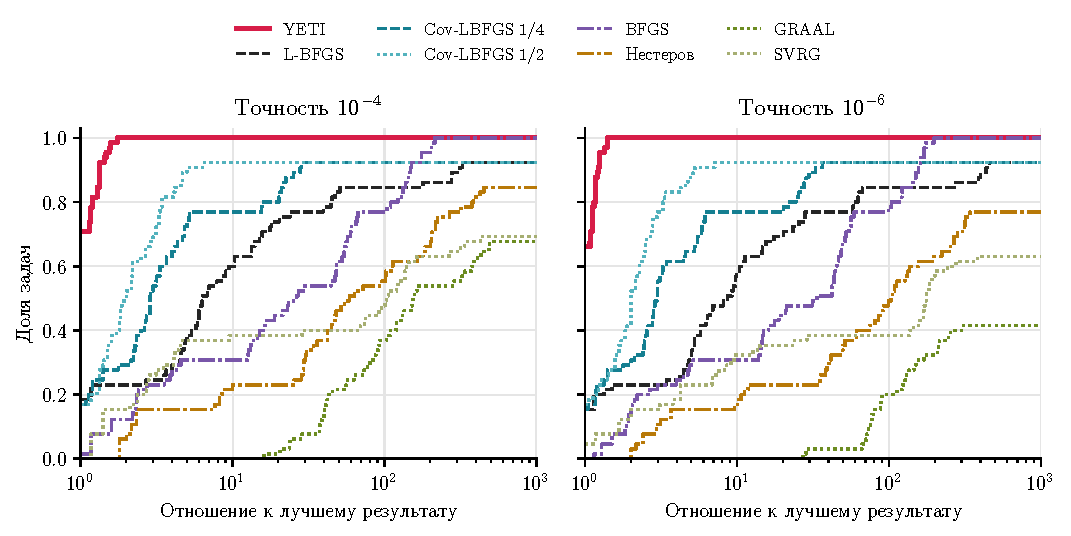
\includegraphics[width=\linewidth]{figures/profiles.pdf}
 \caption{Доля из 65 задач, на которых число запросов не превышает
 лучший результат более чем в $\tau$ раз \citep{dolan2002profiles}. При $\tau=1$ учитываются
 все первые места, включая разделённые; неудачные запуски остаются
 в знаменателе.}
 \label{fig:exp-profiles}
\end{figure}

\begin{table}[!htbp]
 \centering\small
 \setlength{\tabcolsep}{2.3pt}
 \begin{tabular}{@{}lrrrrrrrr@{}}
 \toprule
 Семейство & YETI & L-BFGS & Cov-LBFGS & Cov-LBFGS & BFGS & Нестеров & GRAAL & SVRG\\
 & & (50) & $1/4$ & $1/2$ & & & &\\
 \midrule
 \experimentrows{tables/series65.tex}
 \bottomrule
 \end{tabular}
 \caption{Медиана числа проходов до относительной точности $10^{-6}$
 по пяти экземплярам. «---» означает неудачу хотя бы на одном экземпляре,
 жирным выделен минимум до округления. $\kappa$ --- число обусловленности
 ковариации признаков, $n\times d$ --- число компонент и размерность.}
 \label{tab:exp-series}
\end{table}

Результаты на основном наборе приведены в таблицах~\ref{tab:exp-chains}
и~\ref{tab:exp-glm}. В дополнительных запусках YETI на пяти
синтетических пуассоновских экземплярах медианы числа проходов равны
4, 5 и 5 при $n=2000$, $20000$ и $100000$;
диапазоны --- 4--5, 5--7 и 5--8 соответственно.

\begin{table}[!htbp]
 \centering\small
 \setlength{\tabcolsep}{4pt}
 \begin{tabular}{@{}lrrrrrrrr@{}}
 \toprule
 & \multicolumn{4}{c}{S, длина $T$} & \multicolumn{4}{c}{X, длина $T$}\\
 \cmidrule(lr){2-5}\cmidrule(l){6-9}
 Метод & 8 & 16 & 32 & 64 & 8 & 16 & 32 & 64\\
 \midrule
 \experimentrows{tables/chains.tex}
 \bottomrule
 \end{tabular}
 \caption{Число проходов до относительной точности $10^{-2}$
 на цепочках. Жирным выделен минимум до округления;
 «---» означает, что допуск не достигнут за отведённое число проходов.}
 \label{tab:exp-chains}
\end{table}

\begin{table}[!htbp]
 \centering\small
 \setlength{\tabcolsep}{4pt}
 \begin{tabular}{@{}crrrrrrr@{}}
 \toprule
 & & \multicolumn{3}{c}{До $10^{-2}\widehat\Delta$}
 & \multicolumn{3}{c}{До собственного критерия}\\
 \cmidrule(lr){3-5}\cmidrule(l){6-8}
 Семейство & $T$ & YETI & Без & Случайные & YETI & Без & Случайные\\
 & & & предложений & предложения & & предложений & предложения\\
 \midrule
 \experimentrows{tables/insurance.tex}
 \bottomrule
 \end{tabular}
 \caption{Число проходов при трёх вариантах эвристики.
 Для собственного критерия используется $\varepsilon=10^{-3}\widehat\Delta$.
 «---» означает, что он не выполнен за 200000 проходов.}
 \label{tab:exp-insurance}
\end{table}

\begin{table}[!htbp]
 \centering\small
 \begin{tabular}{@{}lrrrrr@{}}
 \toprule
 & \multicolumn{3}{c}{Синтетические задачи, $n$}
 & Bike & freMTPL2\\
 \cmidrule(lr){2-4}
 Метод & $2000$ & $20000$ & $100000$ & Sharing & freq\\
 \midrule
 \experimentrows{tables/glm.tex}
 \bottomrule
 \end{tabular}
 \caption{Число проходов до относительной точности $10^{-4}$
 на пуассоновских моделях. Обозначения как в табл.~\ref{tab:exp-chains}.}
 \label{tab:exp-glm}
\end{table}
\FloatBarrier

\subsection{Проверка остановки}

На 65 задачах при $\varepsilon=10^{-6}\widehat\Delta$
не менее 90\% запусков завершаются не позднее чем за 37 проходов.
В 63 из 65 запусков YETI останавливается уже в первом эвристическом
блоке. Основной проксимальный шаг понадобился только на двух экземплярах
с редкими признаками при $n=50000$: он выполнен 4 и 8 раз.
На основном наборе все 45 запусков (24 на цепочках и 21 на регрессии)
завершились до первого такого шага.
Рисунок~\ref{fig:exp-certificate} показывает два дополнительных запуска
с более строгим допуском.

\begin{figure}[!htbp]
 \centering
 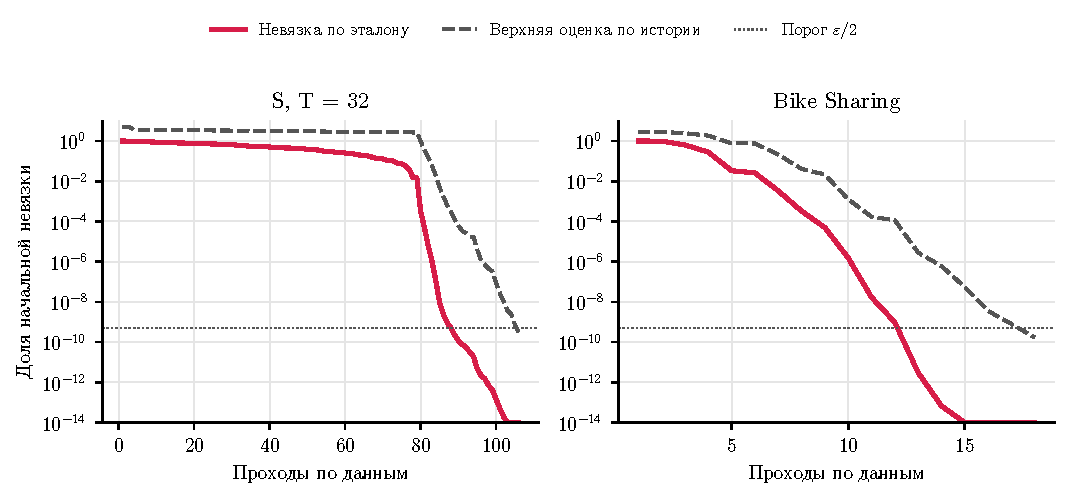
\includegraphics[width=\linewidth]{figures/certificate.pdf}
 \caption{Невязка относительно эталона и её верхняя оценка по истории
 при $\varepsilon=10^{-9}\widehat\Delta$. Все величины делятся на
 $\widehat\Delta$; пунктир --- порог $\varepsilon/2$.
 Значения ниже $10^{-14}$ показаны на нижней границе шкалы.}
 \label{fig:exp-certificate}
\end{figure}

В таблице~\ref{tab:exp-insurance} сопоставлены обычная эвристика,
блок из одного проверочного прохода без предложений и блок, предлагающий
случайные точки допустимого шара. В последнем варианте каждый блок расходует
весь разрешённый лимит: 243--264 прохода.
Общее ограничение составляет 60000 проходов в режиме без предложений
и 200000 --- со случайными предложениями.

Допуск $10^{-2}\widehat\Delta$ достигнут во всех запусках.
Отключение предложений эвристики увеличивает число проходов до допуска
примерно в 41--58 раз, а случайные предложения --- ещё примерно
в 19--54 раза относительно режима без предложений. Таким образом,
в этих опытах основной выигрыш даёт эвристика. Однако её матричные
операции могут быть дорогими, поэтому выигрыш в числе запросов
не обязательно означает такой же выигрыш во времени.
На X при $T=16$ собственный критерий не выполнен за отведённое
число проходов. Ограничение длины блока не устраняет затрат
на бесполезные предложения.
\FloatBarrier

\clearpage
\section{Сводная таблица известных оценок}\label{app:literature}
\enlargethispage{2\baselineskip}
% В узких колонках таблицы формулам разрешено переноситься.
\relpenalty=500 \binoppenalty=700
\providecommand\yes{\textcolor{green!55!black}{\ding{51}}}
\providecommand\no{\textcolor{red!80!black}{\ding{55}}}

\begin{center}
\footnotesize
\captionof{table}{Минимизация суммы: число обращений к оракулу одного слагаемого.}
\label{tab:lit-sum}
\renewcommand\arraystretch{1.0}\setlength\tabcolsep{4pt}
\begin{tabularx}{\linewidth}{@{}P{.18\linewidth}P{.13\linewidth}cP{.14\linewidth}Y@{}}
\toprule
Метод и работа & Гладкость & Выпуклые & Критерий & Оценка\\
\midrule
\multicolumn{5}{@{}l}{\textit{Сумма, $L$-гладкие слагаемые}}\\
SAGA\newline\citet{defazio2014saga} & $L$ & \yes & $\E f(\hat x)-f^\ast\le\varepsilon$
 & $\displaystyle O\Bigl(n+\frac{nF_0+LR^2}{\varepsilon}\Bigr)$\\
Katyusha с AdaptReg\textsuperscript{\dag}\newline\citet{allenzhu2018katyusha} & $L$ & \yes & $\E f(\hat x)-f^\ast\le\varepsilon$
 & $\displaystyle O\Bigl(n\log\frac{F_0}{\varepsilon}+\sqrt{\frac{nLR^2}{\varepsilon}}\Bigr)$\\
Varag\textsuperscript{\ddag}\newline\citet{lan2019varag} & $L$ & \yes & $\E f(\hat x)-f^\ast\le\varepsilon$
 & $\displaystyle O\Bigl(n+n\log\min\Bigl\{n,\frac{D_0}{\varepsilon}\Bigr\}+\sqrt{\frac{nD_0}{\varepsilon}}\Bigr)$\\
Нижняя оценка\textsuperscript{\S}\newline\citet{woodworth2016finite} & $L$ & \yes & $\E f(\hat x)-f^\ast\le\varepsilon$
 & $\displaystyle \Omega\Bigl(n+\sqrt{\frac{nLR^2}{\varepsilon}}\Bigr)$\\
\midrule
\multicolumn{5}{@{}l}{\textit{Одна функция ($n=1$), обобщённая гладкость, оракул полного градиента}}\\
Ускоренный метод\textsuperscript{\P}\newline\citet{tyurin2026accelerated} & sym.\ $(L_0,L_1)$ функции $f$ & \yes & $f(\hat x)-f^\ast\le\varepsilon$
 & $\displaystyle O\Bigl(\sqrt{\frac{L_0R^2}{\varepsilon}}+L_1R\log_+\min\Bigl\{\frac{2L_1^2F_0}{L_0},\frac{2F_0}{\varepsilon}\Bigr\}$\newline
 \hspace*{1em}$\displaystyle{}+\log_+\frac{2F_0}{L_0R^2}\Bigr)$\\
Верхняя и нижняя оценки\textsuperscript{\dag\dag}\newline\citet{rudomanov2026everest} & sym.\ $(L_0,L_1)$ функции $f$ & \yes & $f(\hat x)-f^\ast\le\varepsilon$
 & $\displaystyle\widetilde\Theta\Bigl(\sqrt{\frac{L_0R^2}{\varepsilon}}+L_1R\Bigr)$;\newline
 при $F_0\le4\varepsilon$: $\displaystyle\widetilde\Theta\Bigl(\sqrt{\frac{L_0R^2}{\varepsilon}}+(L_1R)^{2/3}\Bigr)$\\
\midrule
\multicolumn{5}{@{}l}{\textit{Сумма, обобщённая гладкость}}\\
$(L_0,L_1)$-SGD, SGD-PS\textsuperscript{\ddag\ddag}\newline\citet{gorbunov2024methods} & sym.\ $(L_0,L_1)$ каждого $f_i$ & \yes & см.\ прим.~\textsuperscript{\ddag\ddag}
 & $\displaystyle O\Bigl(\frac{L_0R^2}{\varepsilon}\Bigr)$\newline
 при $\delta=0$ (у всех $f_i$ общая точка минимума)\\
$(L_0,L_1)$-SPIDER\textsuperscript{\S\S}\newline\citet{reisizadeh2023variance} & усредн.\ $(L_0,L_1)$ & \no & $\norm{\nabla f(\hat x)}\le\varepsilon$ с вероятностью ${}\ge1/2$
 & $\displaystyle O\Bigl(n+\frac{\sqrt n\,L_0F_0}{\varepsilon^2}\Bigr)$\\
\midrule
\textbf{YETI} и нижняя оценка\textsuperscript{\P\P}\newline\textbf{Эта статья}, теорема~\ref{thm:main} & sym.\ $(L_{0,i},L_1)$ каждого $f_i$ & \yes & $\E f(\hat x)-f^\ast\le\varepsilon$
 & $\displaystyle\widetilde\Theta\Bigl(n\bigl(1+(L_1R)^{2/3}\bigr)+\sqrt{\frac{n(L_0+L_1^2\delta)R^2}{\varepsilon}+n(L_1R)^2}\Bigr)$\\
\bottomrule
\end{tabularx}
\par\smallskip\raggedright\scriptsize
\emph{Обозначения.} $R=\norm{x_0-x^\ast}$, $F_0=f(x_0)-f^\ast$, $\log_+=\max\{\log,0\}$;
$O(\cdot)$ и $\Omega(\cdot)$ скрывают абсолютные константы, $\widetilde\Theta(\cdot)$ ---
ещё и логарифмические множители. Столбец <<Выпуклые>>: \yes{} --- результат получен
для выпуклых $f_i$, \no{} --- выпуклость не предполагается.\par
\emph{Гладкость.} $L$: градиент каждого $f_i$ липшицев с константой~$L$.
sym.: симметричная $(L_0,L_1)$-гладкость \citep[предположение~1.3]{gorbunov2024methods},
$\norm{\nabla g(x)-\nabla g(y)}\le\bigl(L_0+L_1\sup_{u\in[x,y]}\norm{\nabla g(u)}\bigr)\norm{x-y}$
при всех $x,y$; для $C^2$ это равносильно $\norm{\nabla^2g(x)}\le L_0+L_1\norm{\nabla g(x)}$.
Усредн.: усреднённая $(L_0,L_1)$-гладкость \citep[предположение~1(ii)]{reisizadeh2023variance},
$\bigl(\frac1n\sum_{i=1}^n\norm{\nabla f_i(x)-\nabla f_i(y)}^2\bigr)^{1/2}\le\bigl(L_0+L_1\norm{\nabla f(x)}\bigr)\norm{x-y}$
при $\norm{x-y}\le1/L_1$: слагаемые ограничены лишь в среднеквадратичном смысле,
а справа стоит градиент суммы $f$, а не градиенты слагаемых.\par\smallskip
\textsuperscript{\dag}~При $0<\varepsilon\le F_0/2$.\quad
\textsuperscript{\ddag}~$D_0=2F_0+\frac32LR^2$; оценка записана при $D_0\ge\varepsilon$.\quad
\textsuperscript{\dag\dag}~Для детерминированных методов при $L_0R^2\ge\varepsilon$.\par
\textsuperscript{\S}~Для рандомизированных алгоритмов в достаточно большой размерности, на шаре $\norm x\le R$.\par
\textsuperscript{\P}~Результат получен для $\ell$-гладких функций,
$\norm{\nabla^2f(x)}\le\ell(\norm{\nabla f(x)})$: для общей $\ell$ оценка равна
$O\bigl(\sqrt{\ell(0)}\,R/\sqrt\varepsilon+T\bigr)$ с неявным $T$
\citep[следствие~5.3]{tyurin2026accelerated}. Здесь она сведена к $\ell(s)=L_0+L_1s$
\citep[теорема~4.3]{tyurin2026accelerated} при $\bar R=R$, $\Gamma_0=2F_0/R^2$.\par
\textsuperscript{\ddag\ddag}~Число стохастических градиентов до выполнения
$\min_k\E\min\bigl\{\frac{\nu L_0}{4nL_1^2},f(x_k)-f^\ast\bigr\}\le\varepsilon$, где
$\nu=e^{-\nu}$ \citep[теоремы~7.2, 7.3]{gorbunov2024methods}; SGD-PS ещё
требует знать все $\min f_i$.\par
\textsuperscript{\S\S}~При $\varepsilon<L_0/(20L_1)$; здесь $F_0=f(x_0)-\inf f$
\citep[теорема~4]{reisizadeh2023variance}.\par
\textsuperscript{\P\P}~$L_{0,i}$ могут различаться, $\frac1n\sum_iL_{0,i}\le L_0$.
Сложность в смысле определения~\ref{def:oracle}; скрыты множители $\log^2N_0$ (нижняя оценка)
и $\log^2N$ (верхняя). Предположения~\ref{asm:components}--\ref{asm:accuracy}, в том числе $n\ge2$,
$\Delta\ge2\varepsilon$, $L_1^2R^2\delta/\varepsilon\ge3$; случай $\delta=0$ не охватывается.\par
\end{center}

\endgroup
\end{document}
